%%%%%%%%%%%%%%%%%%%%%%%%%%%%%%%%%%%%%%%%%
% Beamer Presentation
% LaTeX Template
% Version 2.0 (March 8, 2022)
%
% This template originates from:
% https://www.LaTeXTemplates.com
%
% Author:
% Vel (vel@latextemplates.com)
%
% License:
% CC BY-NC-SA 4.0 (https://creativecommons.org/licenses/by-nc-sa/4.0/)
%
%%%%%%%%%%%%%%%%%%%%%%%%%%%%%%%%%%%%%%%%%

% ---  ---  ---  ---  ---  ---  ---  ---  ---  ---  ---  ---  ---  ---  ---  ---  ---  ---  ---  ---  ---  ---  ---  ---  ---  ---  ---  ---  ---  ---  ---  ---  ---  ---  ---  ---  ---  ---  ---  ---  ---  ---  ---  --- 
%	PACKAGES AND OTHER DOCUMENT CONFIGURATIONS
% ---  ---  ---  ---  ---  ---  ---  ---  ---  ---  ---  ---  ---  ---  ---  ---  ---  ---  ---  ---  ---  ---  ---  ---  ---  ---  ---  ---  ---  ---  ---  ---  ---  ---  ---  ---  ---  ---  ---  ---  ---  ---  ---  --- 

\documentclass[
	9pt, % Set the default font size, options include: 8pt, 9pt, 10pt, 11pt, 12pt, 14pt, 17pt, 20pt
	%t, % Uncomment to vertically align all slide content to the top of the slide, rather than the default centered
	%aspectratio=169, % Uncomment to set the aspect ratio to a 16:9 ratio which matches the aspect ratio of 1080p and 4K screens and projectors
]{beamer}
% \documentclass[slidestop,compress,mathserif]{beamer}

\graphicspath{{Images/}{./}} % Specifies where to look for included images (trailing slash required)

\usepackage{booktabs} % Allows the use of \toprule, \midrule and \bottomrule for better rules in tables
\usepackage[tight]{subfigure}
\usepackage{multirow}
\usepackage[linesnumbered,titlenumbered,ruled,vlined,commentsnumbered,noend]{algorithm2e}
\newcommand\mycommfont[1]{\footnotesize\ttfamily\textcolor{blue}{#1}}
\SetCommentSty{mycommfont}
\newcommand{\hangcheng}[1]{\textbf{\textcolor{teal}{H. Liu}}}
\newenvironment<>{varblock}[2][\textwidth]{%
  \setlength{\textwidth}{#1}
  \begin{actionenv}#3%
    \def\insertblocktitle{#2}%
    \par%
    \usebeamertemplate{block begin}}
  {\par%
    \usebeamertemplate{block end}%
  \end{actionenv}}

  \definecolor{uibred}{HTML}{db3f3d}
  \definecolor{uibblue}{HTML}{6495ED}
  \definecolor{uibbg}{HTML}{E6E6FA}

  \setbeamercolor{block body}{bg = uibbg}
  \setbeamercolor{block title}{fg=white, bg=uibblue}
% ---  ---  ---  ---  ---  ---  ---  ---  ---  ---  ---  ---  ---  ---  ---  ---  ---  ---  ---  ---  ---  ---  ---  ---  ---  ---  ---  ---  ---  ---  ---  ---  ---  ---  ---  ---  ---  ---  ---  ---  ---  ---  ---  --- 
%	SELECT LAYOUT THEME
% ---  ---  ---  ---  ---  ---  ---  ---  ---  ---  ---  ---  ---  ---  ---  ---  ---  ---  ---  ---  ---  ---  ---  ---  ---  ---  ---  ---  ---  ---  ---  ---  ---  ---  ---  ---  ---  ---  ---  ---  ---  ---  ---  --- 

% Beamer comes with a number of default layout themes which change the colors and layouts of slides. Below is a list of all themes available, uncomment each in turn to see what they look like.

% \usetheme{default}
% \usetheme{AnnArbor}
% \usetheme{Antibes}
% \usetheme{Bergen}
% \usetheme{Berkeley}
% \usetheme{Berlin} %y
% \usetheme{Boadilla} %y
% \usetheme{CambridgeUS}
% \usetheme{Copenhagen}
% \usetheme{Darmstadt}
% \usetheme{Dresden} %y
% \usetheme{Frankfurt}
\usetheme{Goettingen} %y
% \usetheme{Hannover}
% \usetheme{Ilmenau}
% \usetheme{JuanLesPins}
% \usetheme{Luebeck}
% \usetheme{Madrid}
% \usetheme{Malmoe}
% \usetheme{Marburg}
% \usetheme{Montpellier}
% \usetheme{PaloAlto}
% \usetheme{Pittsburgh}
% \usetheme{Rochester}
% \usetheme{Singapore}
% \usetheme{Szeged} %y
% \usetheme{Warsaw}

% ---  ---  ---  ---  ---  ---  ---  ---  ---  ---  ---  ---  ---  ---  ---  ---  ---  ---  ---  ---  ---  ---  ---  ---  ---  ---  ---  ---  ---  ---  ---  ---  ---  ---  ---  ---  ---  ---  ---  ---  ---  ---  ---  --- 
%	SELECT COLOR THEME
% ---  ---  ---  ---  ---  ---  ---  ---  ---  ---  ---  ---  ---  ---  ---  ---  ---  ---  ---  ---  ---  ---  ---  ---  ---  ---  ---  ---  ---  ---  ---  ---  ---  ---  ---  ---  ---  ---  ---  ---  ---  ---  ---  --- 

% Beamer comes with a number of color themes that can be applied to any layout theme to change its colors. Uncomment each of these in turn to see how they change the colors of your selected layout theme.

%\usecolortheme{albatross}
%\usecolortheme{beaver}
%\usecolortheme{beetle}
%\usecolortheme{crane}
%\usecolortheme{dolphin}
%\usecolortheme{dove}
%\usecolortheme{fly}
%\usecolortheme{lily}
%\usecolortheme{monarca}
%\usecolortheme{seagull}
%\usecolortheme{seahorse}
%\usecolortheme{spruce}
%\usecolortheme{whale}
%\usecolortheme{wolverine}

% ---  ---  ---  ---  ---  ---  ---  ---  ---  ---  ---  ---  ---  ---  ---  ---  ---  ---  ---  ---  ---  ---  ---  ---  ---  ---  ---  ---  ---  ---  ---  ---  ---  ---  ---  ---  ---  ---  ---  ---  ---  ---  ---  --- 
%	SELECT FONT THEME & FONTS
% ---  ---  ---  ---  ---  ---  ---  ---  ---  ---  ---  ---  ---  ---  ---  ---  ---  ---  ---  ---  ---  ---  ---  ---  ---  ---  ---  ---  ---  ---  ---  ---  ---  ---  ---  ---  ---  ---  ---  ---  ---  ---  ---  --- 

% Beamer comes with several font themes to easily change the fonts used in various parts of the presentation. Review the comments beside each one to decide if you would like to use it. Note that additional options can be specified for several of these font themes, consult the beamer documentation for more information.

\usefonttheme{default} % Typeset using the default sans serif font
%\usefonttheme{serif} % Typeset using the default serif font (make sure a sans font isn't being set as the default font if you use this option!)
%\usefonttheme{structurebold} % Typeset important structure text (titles, headlines, footlines, sidebar, etc) in bold
%\usefonttheme{structureitalicserif} % Typeset important structure text (titles, headlines, footlines, sidebar, etc) in italic serif
%\usefonttheme{structuresmallcapsserif} % Typeset important structure text (titles, headlines, footlines, sidebar, etc) in small caps serif

% ---  ---  ---  ---  ---  ---  ---  ---  ---  ---  ---  ---  ---  ---  ---  ---  ---  ---  ---  ---  ---  ---  ---  --- 

%\usepackage{mathptmx} % Use the Times font for serif text
\usepackage{palatino} % Use the Palatino font for serif text

%\usepackage{helvet} % Use the Helvetica font for sans serif text
\usepackage[default]{opensans} % Use the Open Sans font for sans serif text
%\usepackage[default]{FiraSans} % Use the Fira Sans font for sans serif text
%\usepackage[default]{lato} % Use the Lato font for sans serif text

% ---  ---  ---  ---  ---  ---  ---  ---  ---  ---  ---  ---  ---  ---  ---  ---  ---  ---  ---  ---  ---  ---  ---  ---  ---  ---  ---  ---  ---  ---  ---  ---  ---  ---  ---  ---  ---  ---  ---  ---  ---  ---  ---  --- 
%	SELECT INNER THEME
% ---  ---  ---  ---  ---  ---  ---  ---  ---  ---  ---  ---  ---  ---  ---  ---  ---  ---  ---  ---  ---  ---  ---  ---  ---  ---  ---  ---  ---  ---  ---  ---  ---  ---  ---  ---  ---  ---  ---  ---  ---  ---  ---  --- 

% Inner themes change the styling of internal slide elements, for example: bullet points, blocks, bibliography entries, title pages, theorems, etc. Uncomment each theme in turn to see what changes it makes to your presentation.

%\useinnertheme{default}
\useinnertheme{circles}
%\useinnertheme{rectangles}
%\useinnertheme{rounded}
%\useinnertheme{inmargin}

% ---  ---  ---  ---  ---  ---  ---  ---  ---  ---  ---  ---  ---  ---  ---  ---  ---  ---  ---  ---  ---  ---  ---  ---  ---  ---  ---  ---  ---  ---  ---  ---  ---  ---  ---  ---  ---  ---  ---  ---  ---  ---  ---  --- 
%	SELECT OUTER THEME
% ---  ---  ---  ---  ---  ---  ---  ---  ---  ---  ---  ---  ---  ---  ---  ---  ---  ---  ---  ---  ---  ---  ---  ---  ---  ---  ---  ---  ---  ---  ---  ---  ---  ---  ---  ---  ---  ---  ---  ---  ---  ---  ---  --- 

% Outer themes change the overall layout of slides, such as: header and footer lines, sidebars and slide titles. Uncomment each theme in turn to see what changes it makes to your presentation.

%\useoutertheme{default}
%\useoutertheme{infolines}
%\useoutertheme{miniframes}
%\useoutertheme{smoothbars}
%\useoutertheme{sidebar}
%\useoutertheme{split}
%\useoutertheme{shadow}
%\useoutertheme{tree}
%\useoutertheme{smoothtree}

%\setbeamertemplate{footline} % Uncomment this line to remove the footer line in all slides
%\setbeamertemplate{footline}[page number] % Uncomment this line to replace the footer line in all slides with a simple slide count

%\setbeamertemplate{navigation symbols}{} % Uncomment this line to remove the navigation symbols from the bottom of all slides

% ---  ---  ---  ---  ---  ---  ---  ---  ---  ---  ---  ---  ---  ---  ---  ---  ---  ---  ---  ---  ---  ---  ---  ---  ---  ---  ---  ---  ---  ---  ---  ---  ---  ---  ---  ---  ---  ---  ---  ---  ---  ---  ---  --- 
%	PRESENTATION INFORMATION
% ---  ---  ---  ---  ---  ---  ---  ---  ---  ---  ---  ---  ---  ---  ---  ---  ---  ---  ---  ---  ---  ---  ---  ---  ---  ---  ---  ---  ---  ---  ---  ---  ---  ---  ---  ---  ---  ---  ---  ---  ---  ---  ---  --- 

\title[CSL@CQU]{Summary Of Works During Ph.D. Candidate} % The short title in the optional parameter appears at the bottom of every slide, the full title in the main parameter is only on the title page

% \subtitle{Summary In Ph.D. Candidate} % Presentation subtitle, remove this command if a subtitle isn't required

\author[Hangcheng Liu]{Hangcheng Liu} % Presenter name(s), the optional parameter can contain a shortened version to appear on the bottom of every slide, while the main parameter will appear on the title slide

\institute[CQU]{Cyber Security Laboratory, Chongqing University \\ \smallskip hcliu@cqu.edu.cn} % Your institution, the optional parameter can be used for the institution shorthand and will appear on the bottom of every slide after author names, while the required parameter is used on the title slide and can include your email address or additional information on separate lines

\date[\today]{\today} % Presentation date or conference/meeting name, the optional parameter can contain a shortened version to appear on the bottom of every slide, while the required parameter value is output to the title slide

% ---  ---  ---  ---  ---  ---  ---  ---  ---  ---  ---  ---  ---  ---  ---  ---  ---  ---  ---  ---  ---  ---  ---  ---  ---  ---  ---  ---  ---  ---  ---  ---  ---  ---  ---  ---  ---  ---  ---  ---  ---  ---  ---  --- 

\begin{document}

% ---  ---  ---  ---  ---  ---  ---  ---  ---  ---  ---  ---  ---  ---  ---  ---  ---  ---  ---  ---  ---  ---  ---  ---  ---  ---  ---  ---  ---  ---  ---  ---  ---  ---  ---  ---  ---  ---  ---  ---  ---  ---  ---  --- 
%	TITLE SLIDE
% ---  ---  ---  ---  ---  ---  ---  ---  ---  ---  ---  ---  ---  ---  ---  ---  ---  ---  ---  ---  ---  ---  ---  ---  ---  ---  ---  ---  ---  ---  ---  ---  ---  ---  ---  ---  ---  ---  ---  ---  ---  ---  ---  --- 

\begin{frame}
	\titlepage % Output the title slide, automatically created using the text entered in the PRESENTATION INFORMATION block above
\end{frame}

% ---  ---  ---  ---  ---  ---  ---  ---  ---  ---  ---  ---  ---  ---  ---  ---  ---  ---  ---  ---  ---  ---  ---  ---  ---  ---  ---  ---  ---  ---  ---  ---  ---  ---  ---  ---  ---  ---  ---  ---  ---  ---  ---  --- 
%	TABLE OF CONTENTS SLIDE
% ---  ---  ---  ---  ---  ---  ---  ---  ---  ---  ---  ---  ---  ---  ---  ---  ---  ---  ---  ---  ---  ---  ---  ---  ---  ---  ---  ---  ---  ---  ---  ---  ---  ---  ---  ---  ---  ---  ---  ---  ---  ---  ---  --- 

% The table of contents outputs the sections and subsections that appear in your presentation, specified with the standard \section and \subsection commands. You may either display all sections and subsections on one slide with \tableofcontents, or display each section at a time on subsequent slides with \tableofcontents[pausesections]. The latter is useful if you want to step through each section and mention what you will discuss.

\begin{frame}
	\frametitle{Presentation Overview} % Slide title, remove this command for no title
	% Contents
	\tableofcontents  % Output the table of contents (all sections on one slide)
	%\tableofcontents[pausesections] % Output the table of contents (break sections up across separate slides)
\end{frame}

% ---  ---  ---  ---  ---  ---  ---  ---  ---  ---  ---  ---  ---  ---  ---  ---  ---  ---  ---  ---  ---  ---  ---  ---  ---  ---  ---  ---  ---  ---  ---  ---  ---  ---  ---  ---  ---  ---  ---  ---  ---  ---  ---  --- 
%	PRESENTATION BODY SLIDES
% ---  ---  ---  ---  ---  ---  ---  ---  ---  ---  ---  ---  ---  ---  ---  ---  ---  ---  ---  ---  ---  ---  ---  ---  ---  ---  ---  ---  ---  ---  ---  ---  ---  ---  ---  ---  ---  ---  ---  ---  ---  ---  ---  --- 

\section{Self-Introduction} % Sections are added in order to organize your presentation into discrFete blocks, all sections and subsections are automatically output to the table of contents as an overview of the talk but NOT output in the presentation as separate slides
\subsection{Education}
% ---  ---  ---  ---  ---  ---  ---  ---  ---  ---  ---  ---  ---  ---  ---  ---  ---  ---  ---  ---  ---  ---  ---  --- 
\begin{frame}
	\frametitle{Education}
	% \begin{columns}[c] % The "c" option specifies centered vertical alignment while the "t" option is used for top vertical alignment
	% 	\begin{column}{0.45\textwidth} % Left column width
	% 		\textbf{Heading}
	% 		\begin{enumerate}
	% 			\item Statement
	% 			\item Explanation
	% 			\item Example
	% 		\end{enumerate}
	% 	\end{column}
	% 	\begin{column}{0.5\textwidth} % Right column width
	% 		Lorem ipsum dolor sit amet, consectetur adipiscing elit. Integer lectus nisl, ultricies in feugiat rutrum, porttitor sit amet augue. Aliquam ut tortor mauris. Sed volutpat ante purus, quis accumsan dolor.
	% 	\end{column}
	% \end{columns}
	\begin{columns}[c]
		\begin{column}{\textwidth}
			% \textbf{Education}
			\begin{itemize}
				\item \textbf{Sep. 2018 --- Now:} Ph.D. candidate in computer science and technology, \textit{Chongqing University,} China
				\item \textbf{Sep. 2017 --- Jun. 2018:} Study in computer science and technology, \textit{Chongqing University,} China
				\item \textbf{Sep. 2018 --- Jun. 2017:} B.E. in information security, \textit{Chongqing University,} China
			\end{itemize}
		\end{column}
	\end{columns}
\end{frame}

\subsection{Main Research Direction}
\begin{frame}
	\frametitle{Main Research Direction}
	{\LARGE \textbf{Adversarial Attacks In Deep Learning}}

	\textbf{Supervisor:} Prof. Tao XIANG

	\vfill
	\begin{figure}
		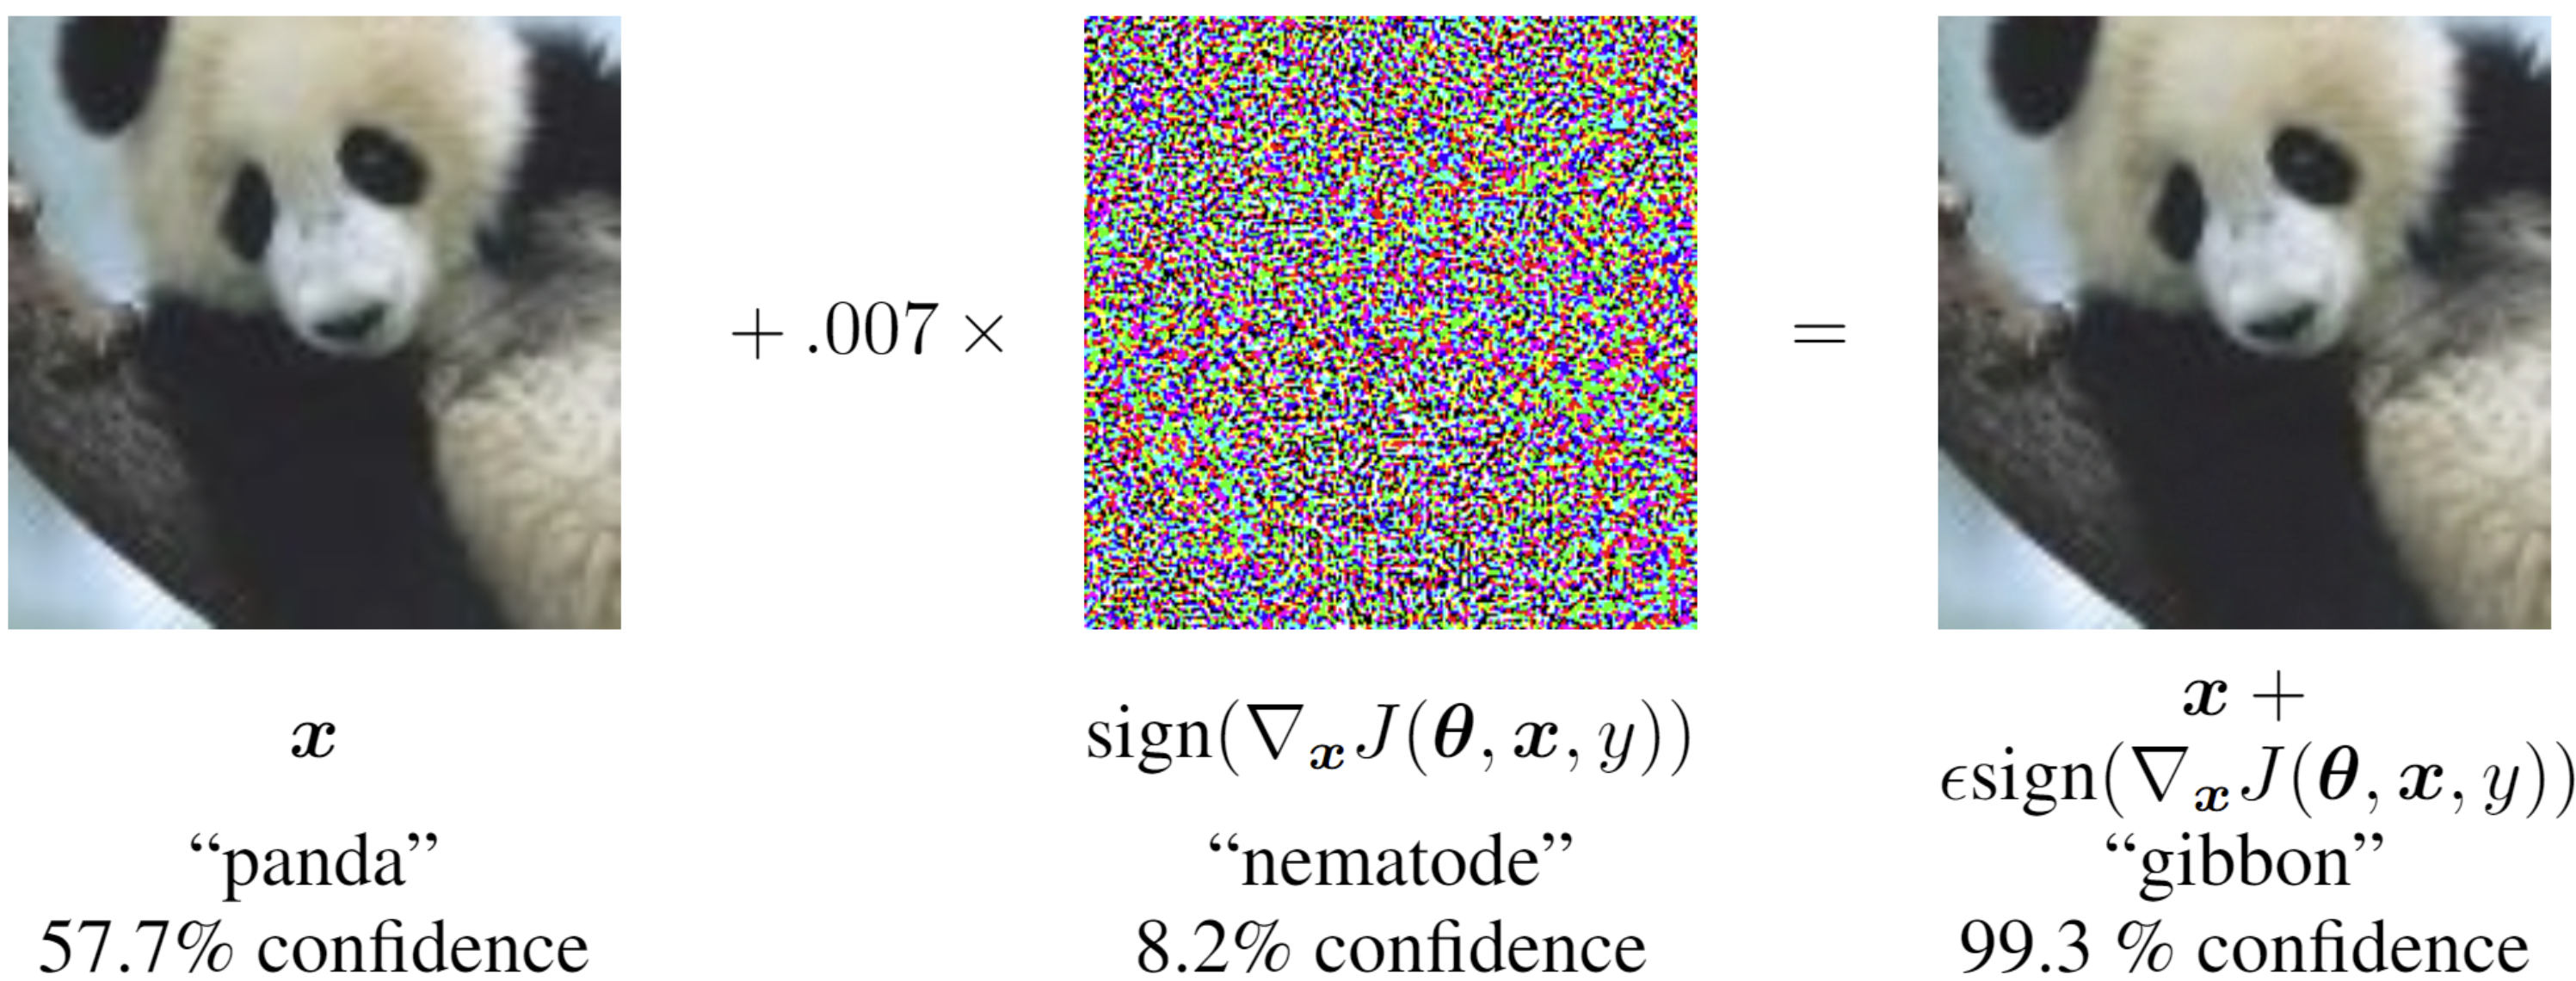
\includegraphics[width=0.8\linewidth]{ae.png}
		\caption{Adversarial example \footnote{Source of Image: Ian J. Goodfellow et al.,``Explaining and harnessing adversarial example,'' ICLR, 2015.}.}
	\end{figure}
\end{frame}

\section{Research During Ph.D.}
\subsection{Publications}
\begin{frame}
	\frametitle{Publications on Security Deep Learning}
	\begin{columns}[c]
		\begin{column}{\textwidth}
			\begin{itemize}
			\item T. Xiang, \hangcheng, S. Guo, H. Liu, and T. Zhang, ``Text's armor: Optimized local adversarial perturbation against scene text editing attacks,'' \emph{Proceedings of ACM International Conference on Multimedia,} 2022. \textbf{CCF Rank A}
			\item \hangcheng, T. Xiang, S. Guo, T. Zhang, and X. Liao, ``Erase and repair: An efficient box-free removal attack on deep hiding,'' \emph{IEEE Transactions on Information Forensics \& Security,} 2022. \textbf{JCR Q1, CCF Rank A} under review
			\item T. Xiang, \hangcheng, S. Guo, Y. Gan, W. He, and X. Liao, ``Towards query efficient black-box attacks: A universal dual transferability-Based framework,'' \emph{ACM Transactions on Intelligent Systems and Technology,} 2022. \textbf{JCR Q1} under review
			\item T. Xiang, \hangcheng, S. Guo, Y, Gan, and X. Liao, ``EGM: An efficient generative model for unrestricted adversarial examples,'' \emph{ACM Transactions on Sensor Networks}, 2022. \textbf{JCR Q3, CCF B}	
			\item S. Guo, S. Geng, T. Xiang, \hangcheng, and R. Hou. ``ELAA: An efficient local adversarial attack using model interpreters,'' \emph{International Journal of Intelligent Systems}, 2021. \textbf{JCR Q1, CCF Rank C}
			% \item T. Xiang, \hangcheng, S. Guo, T. Zhang, ``PEEL: A provable removal attack on deep hiding'' \emph{arXiv preprint arXiv:2106.02779,} 2021. 
			\end{itemize}
		\end{column}
	\end{columns}
\end{frame}


\subsection{Text's Armor}
\begin{frame}
	\frametitle{Text's Armor \footnote{Text's armor: Optimized local adversarial perturbation against scene text editing attacks. ACM MM, 2022.} --- Introduction}
	\begin{block}{Background \& Motivation}
		\begin{figure}
			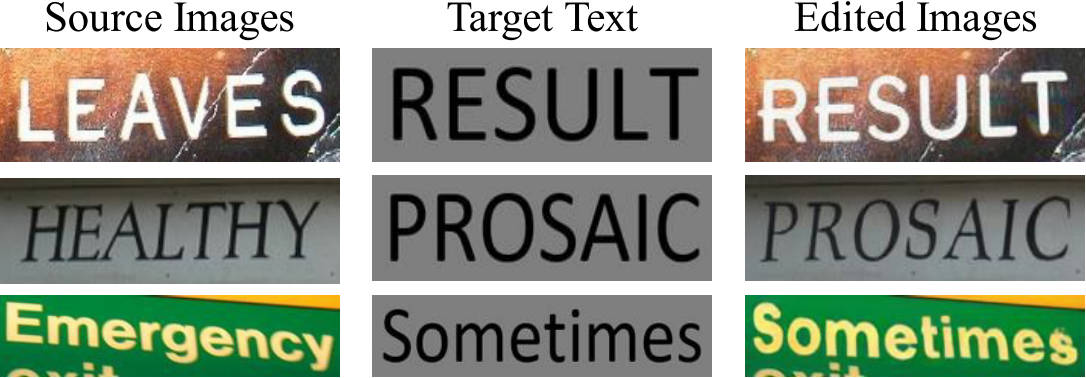
\includegraphics[width=0.5\linewidth]{1.jpg}
			% \caption{Examples of STE.}
		\end{figure}
		\begin{columns}[c]
			\begin{column}{\textwidth}
				\begin{itemize}
				\item DNNs-based scene text editing (STE) can replace source text in images naturally
				\item The abuse of such tools will lead to the proliferation of forgery
				\item DNNs' weakness to adversarial perturbations
				\end{itemize}
			\end{column}
		\end{columns}
	\end{block}
	\begin{block}{Goals of This Paper}
		\begin{columns}[c]
			\begin{column}{\textwidth}
				\begin{itemize}
				\item Prevent malicious editing while preserving the visual quality of source images
				\item Provide fine-grained defenses
				\end{itemize}
			\end{column}
		\end{columns}
	\end{block}
\end{frame}
\begin{frame}
	\frametitle{Text's Armor --- Methodology}
	\begin{columns}[c]
		\begin{column}{0.48\textwidth}
			\begin{block}{Processes in STE Attacks}
				\begin{enumerate}
						\item Text location
						\item Background inpainting
						\item Text style parsing
						\item Fake image generation
				\end{enumerate}
			\end{block}
		\end{column}

		\begin{column}{0.48\textwidth}
			\begin{block}{Precise Defense Goals}
				\begin{enumerate}
						\item Text hiding
						\item Text preservation
						\item Inconsistent text style
						\item Distortion in fake images
				\end{enumerate}	
			\end{block}
		\end{column}
	\end{columns}
	\begin{block}{Framework}
		\begin{figure}
			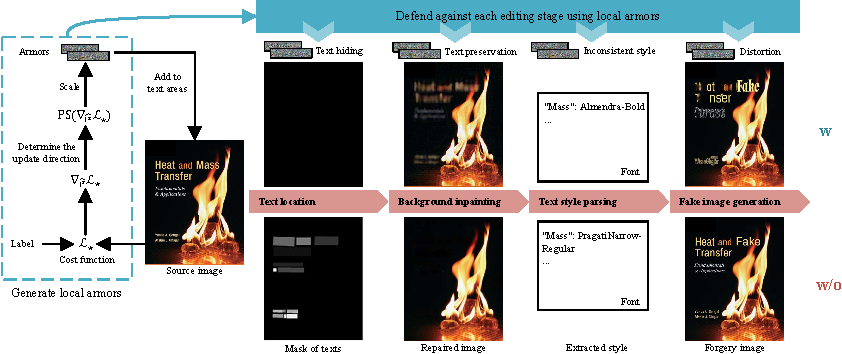
\includegraphics[width=0.85\textwidth]{frame_text_armor.pdf}
		\end{figure}
	\end{block}
\end{frame}
\begin{frame}
	\frametitle{Text's Armor --- Experiments}
	\textbf{Subjective Evaluation}
		\begin{table}[t]
			\centering
			\setlength{\belowcaptionskip}{0 cm}
			% \setlength{\belowcaptionskip}{-0.2 cm}
			\caption{Derendering}
			\resizebox*{\linewidth}{!}{
		\begin{tabular}{cccccccccc}
			\toprule
			\multirow{3}[5]{*}{Method} & \multicolumn{8}{c}{Stage}                                     & \multirow{3}[5]{*}{w/o} \\
			\cmidrule{2-9}      & \multirow{2}[3]{*}{Location} & \multirow{2}[3]{*}{Inpainting} & \multicolumn{5}{c}{Parsing}     & \multirow{2}[3]{*}{Combine} &  \\
			\cmidrule{4-8}      &       &   & Font    & Border-V & Border-E & Shadow-V  & Shadow-E &       &  \\ \midrule
			PS-M-BIM & 100.00\% & 67.58\% & 77.17\% & 21.01\% & 89.27\% & 27.85\% & 93.15\% & 95.89\% & \multirow{2}[1]{*}{10.50\%} \\
			PS-M-PGD & 100.00\% & 64.84\% & 78.54\% & 22.83\% & 89.95\% & 31.51\% & 93.61\% & 97.21\% & \\
			\bottomrule
			\end{tabular}%
			}
			\label{tab:sub-der}%
			\vspace{-0.5cm}
		  \end{table}%
		
		\begin{table}[t]
			\centering
			% \setlength{\abovecaptionskip}{0.cm}

			\caption{SRNet}
			\resizebox*{0.9\linewidth}{!}{
		\begin{tabular}{cccccccc}
			\toprule
			\multirow{3}[5]{*}{Method} & \multirow{3}[5]{*}{$\mathcal{L}_{b}$} & \multicolumn{4}{c}{Stage}     &       & \multirow{3}[5]{*}{w/o} \\
			\cmidrule{3-7}      &       & \multirow{2}[3]{*}{Inpainting} & \multicolumn{2}{c}{Parsing} & \multirow{2}[3]{*}{Generation} & \multirow{2}[3]{*}{Combine} &  \\
			\cmidrule{4-5}      &       &       & Skeleton & Foreground &       &       &  \\ \midrule
			\multirow{2}[1]{*}{PS-M-BIM} & $-\|i^s-o^b\|_1$  & 81.67\% & \multirow{2}[1]{*}{80.83\%} & \multirow{2}[1]{*}{97.67\%} & \multirow{2}[1]{*}{45.33\%} & 50.67\% & \multirow{4}[3]{*}{18.33\%} \\
				  & $\|t^b-o^b\|_1$    & 88.67\% &       &       &       & 85.67\% &  \\
			\cmidrule{1-7}\multirow{2}[2]{*}{PS-M-PGD} & $-\|i^s-o^b\|_1$  & 79.00\% & \multirow{2}[2]{*}{80.33\%} & \multirow{2}[2]{*}{95.83\%} & \multirow{2}[2]{*}{59.50\%} & 66.33\% &  \\
				  & $\|t^b-o^b\|_1$    & 82.17\% &       &       &       & 87.33\% &  \\
			\bottomrule
			\end{tabular}%
			}
			\label{tab:sub-srn}
		\end{table}%
		\alert{Our defense successfully defeats against existing STE attacks since human can easily identify the editing results as \textbf{FALSE} even without professional knowledge after adopting our defense!}
\end{frame}
\begin{frame}
	\frametitle{Text's Armor --- Experiments}
	\textbf{Evaluation in A Black-Box Setting}
	\begin{block}{Portrait Transferability}
		\alert{Perturbation generated for \textbf{Phase A} can also mislead \textbf{Phase B} in the same STE attack.}
		\begin{table}[t]
			\centering
			% \caption{Portrait transferability of different stages}
			\resizebox*{0.6\linewidth}{!}{
			% Table generated by Excel2LaTeX from sheet 'transferability'
		% Table generated by Excel2LaTeX from sheet 'transferability'
		\begin{tabular}{ccccc}
			\toprule
			\multirow{2}[3]{*}{Stage} & RT    & \multicolumn{2}{c}{Acc} & $L_1$ \\
			\cmidrule{2-5}      & Location & Font  & Border-E & Shadow-E \\
			\midrule
			Location & 0.002  & 0.463  & 0.043  & 2.414  \\
			Font  & 0.812  & 0.003  & 0.023  & 2.436  \\
			Border-E & 0.708  & 0.080  & 0.003  & 3.113  \\
			Shadow-E & 0.559  & 0.180  & 0.004  & 7.994  \\
			\bottomrule
			\end{tabular}%
		
			  }
			\label{tab:pt}%
		  \end{table}%
		 
	\end{block}
	\begin{block}{Landscape Transferability}
		\alert{Perturbation generated for \textbf{Attack A} can also affect \textbf{Attack B}.}
		\begin{figure}
			% \setlength{\abovecaptionskip}{0.cm}
			\centering
			\resizebox*{0.5\linewidth}{!}{
				\subfigure[$\hat{i^s}$ for SRNet]{
					\begin{minipage}[b]{0.33\linewidth}
						% 
\includegraphics[width=\linewidth]{00195_is.jpg}
		
						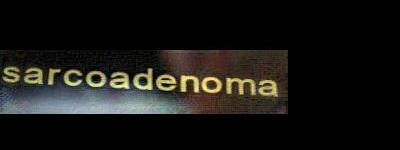
\includegraphics[width=\linewidth]{00265_is.jpg}
		
						% 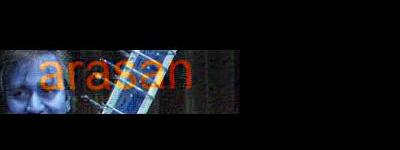
\includegraphics[width=\linewidth]{00282_is.jpg}
		
						% 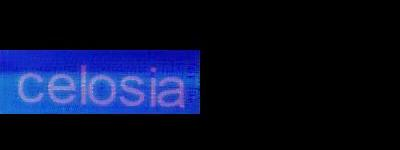
\includegraphics[width=\linewidth]{00274_is.jpg}
					\end{minipage}%
					\label{fig:trans:a}}
			\subfigure[Location in Derendering (w/o)]{
					\begin{minipage}[b]{0.33\linewidth}
						% 
\includegraphics[width=\linewidth]{00195_m.jpg}
		
						
\includegraphics[width=\linewidth]{00265_m.jpg}
		
						% 
\includegraphics[width=\linewidth]{00282_m.jpg}
		
						% 
\includegraphics[width=\linewidth]{00274_m.jpg}
					\end{minipage}%
					\label{fig:trans:b}}
			\subfigure[Location in Derendering (w)]{
					\begin{minipage}[b]{0.33\linewidth}
						% 
\includegraphics[width=\linewidth]{00195_m1.jpg}
		
						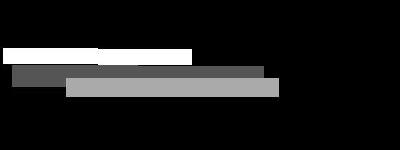
\includegraphics[width=\linewidth]{00265_m1.jpg}
		
						% 
\includegraphics[width=\linewidth]{00282_m1.jpg}
		
						% 
\includegraphics[width=\linewidth]{00274_m1.jpg}
					\end{minipage}%
					\label{fig:trans:c}}
			}
			% \caption{Landscape transferability. (a) Protected source images. (b) Text masks of the original source images. (c) Text masks of protected source images}
			\label{fig:trans}
			% \vspace{-0.5cm}
		\end{figure}
	\end{block}
	\alert{Portrait and landscape transferabilities ensure the practicability of our defense in the real world.}
\end{frame}

\subsection{EGM}
\begin{frame}
	\frametitle{EGM \footnote{EGM: An efficient generative model for unrestricted adversarial examples. TOSN, 2022.} --- Introduction}
	\begin{block}{Background \& Motivation}
		\textbf{Perturbation-based V.S Unrestricted} \footnote{Y. Song et al. ``Constructing Unrestricted Adversarial Examples with Generative Models,'' NeurIPS, 2018} \textbf{Adversarial Example}

		$A_p \triangleq \{x\in \mathcal{O}\,|\,\exists x' \in \mathcal{T},\|x-x'\|\leq\epsilon\wedge f(x')=o(x')=o(x)\neq f(x)\}$

		$A_u \triangleq \{x\in \mathcal{O}\,|\, o(x)\neq f(x)\}$  
		\\
		\textbf{In unrestricted attacks}
		\begin{itemize}
			\item Choose start points freely, i.e., higher flexibility and aggressiveness
			\item It is no longer necessary to collect and store clean samples
		\end{itemize}
		\textbf{\alert{However}}
		\begin{itemize}
			\item Time-consuming
			\item Low attack success rate
		\end{itemize}
	\end{block}
	\begin{block}{Goals of This Paper}
		\begin{itemize}
			\item Improve the generation efficiency of UAE
			\item Improve the attack success rate
		\end{itemize}
	\end{block}
\end{frame}
\begin{frame}
	\frametitle{EGM --- Methodology}
	\begin{columns}[c]
		\begin{column}{0.48\textwidth}
			\begin{block}{Generation Efficiency}
				Use a generative model to generate UAE from noises in one forward calculation. \alert{However, it is hard to train the model in a normal GAN manner due to conflicting gradients \footnote{I. Dunn et al. "Adaptive generation of unrestricted adversarial inputs," Arxiv, 2019.}}
			\end{block}
		\end{column}

		\begin{column}{0.48\textwidth}
			\begin{block}{Attack Success Rate}
				Design an adversarial label augmentation (ALA) strategy to provide dynamic labels that encourage the model to search in different directions and skip local optimization. 
				\bigskip
				\bigskip
				\bigskip
				% \\
			\end{block}
		\end{column}
	\end{columns}
	
	
	% \textbf{Generation efficiency:} generate unrestricted adversarial in one forward calculation $\rightarrow$ a generative model.

	% \textbf{Attack success rate:} design an adversarial label augmentation strategy to provide dynamic labels that encourage the model to search in different directions and skip local optimization. 

	\begin{block}{Framework}
		\begin{figure}
			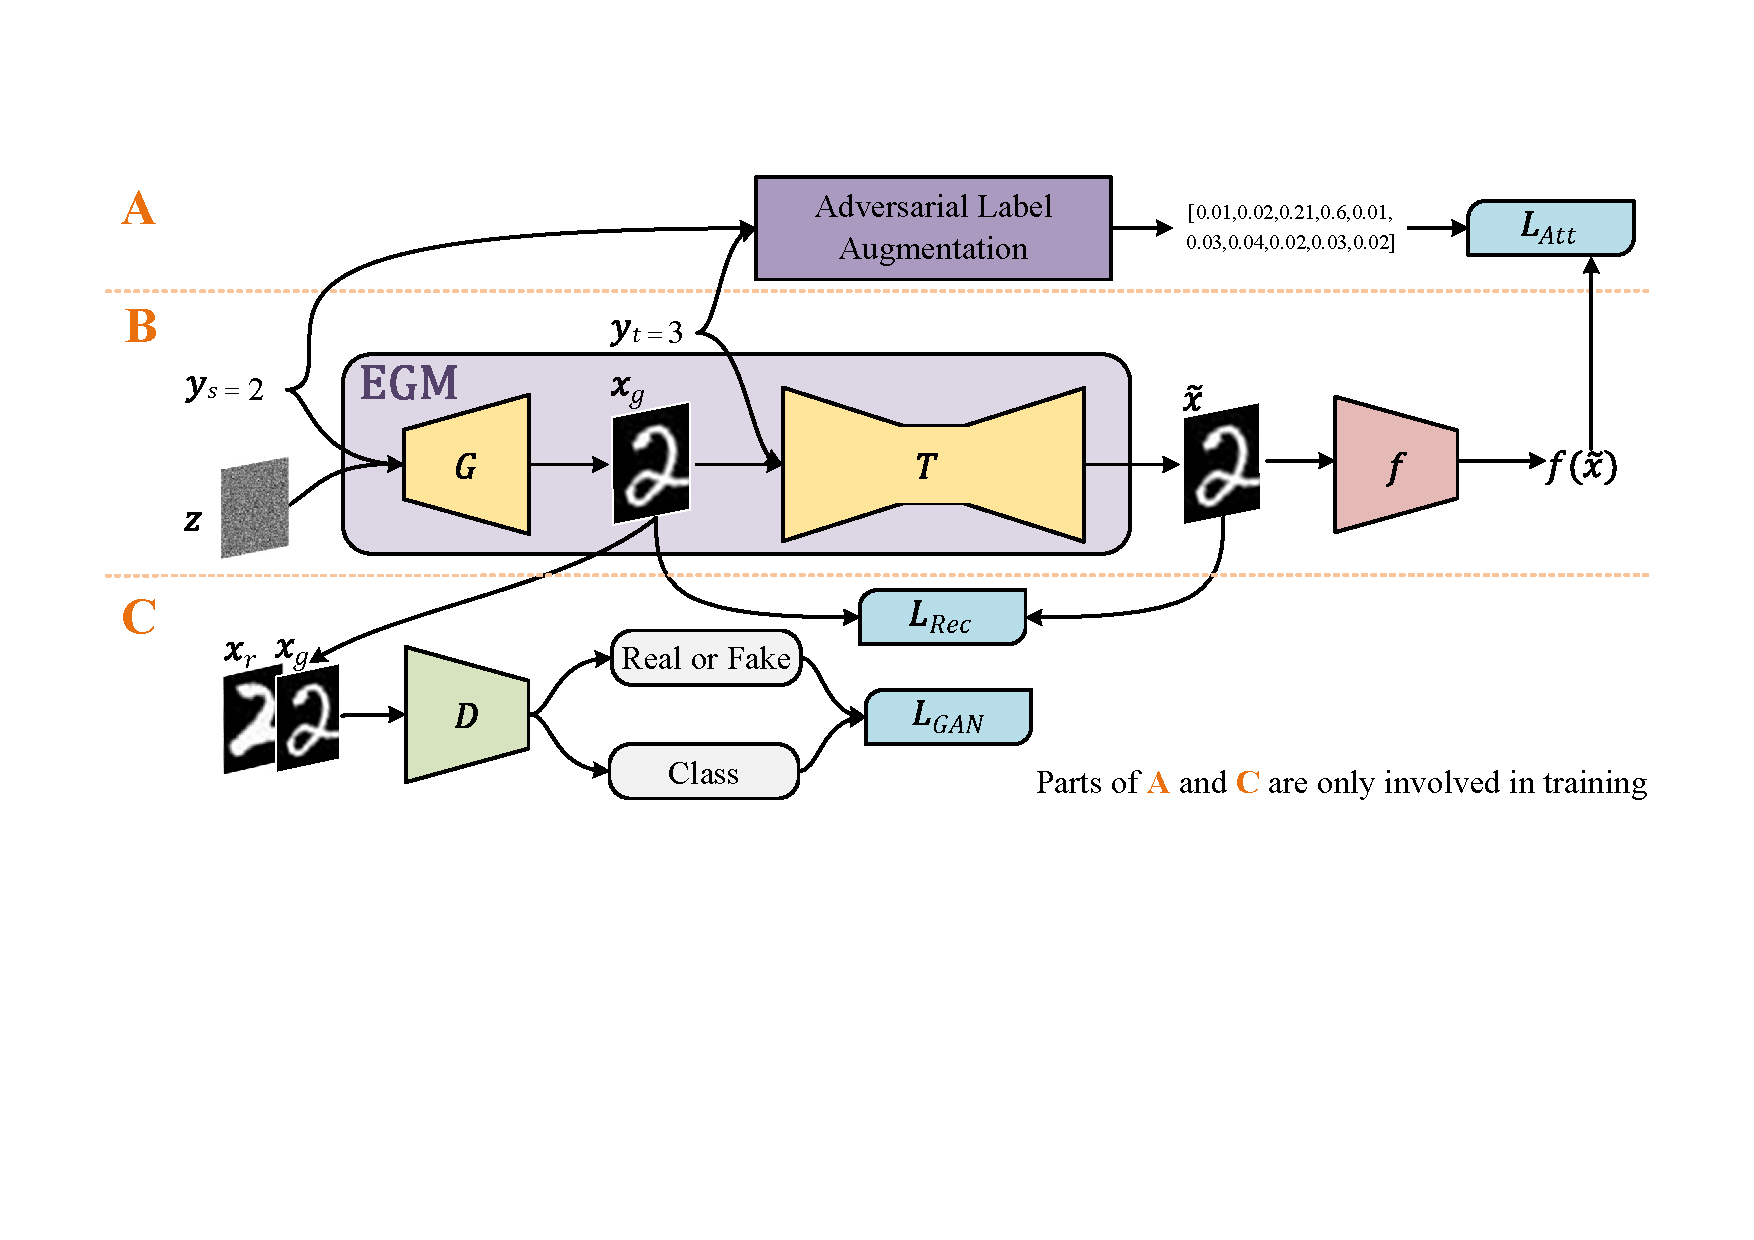
\includegraphics[width=0.75\linewidth]{frame_egm.pdf}
			% \caption{Framework of EGM}
		\end{figure}
	\end{block}

\end{frame}
% \begin{frame}
% 	\frametitle{EGM --- Experiments}
% 	\textbf{Evaluation of Efficiency}
% 	\begin{table}[tbp]
% 		\renewcommand{\arraystretch}{1.2}
% 		\centering
% 		% \caption{Run time of FGSM, ATN, EGM, and USong to produce 1000 adversarial examples on MNIST}
% 		\begin{tabular}{|c|c|r|}
% 			\hline
% 			Type                          & Method & Time (s)  \\ \hline
% 			\multirow{2}{*}{Perturbation-based}            & FGSM    & 0.034    \\ \cline{2-3}
% 			& ATN    & 0.076 \\ \hline
% 			\multirow{2}{*}{Unrestricted} & EGM    & 0.360     \\
% 			\cline{2-3}
% 			& USong  & 32.052    \\ \hline
% 		\end{tabular}
% 		\label{tb:efficency}
% 	\end{table}
% \end{frame}
\begin{frame}
	\frametitle{EGM --- Experiments}
	\textbf{Evaluation of Efficiency}
	\begin{table}[tbp]
		\renewcommand{\arraystretch}{1.2}
		\centering
		% \caption{Run time of FGSM, ATN, EGM, and USong to produce 1000 adversarial examples on MNIST}
		\begin{tabular}{|c|c|r|}
			\hline
			Type                          & Method & Time (s)  \\ \hline
			\multirow{2}{*}{Perturbation-based}            & FGSM    & 0.034    \\ \cline{2-3}
			& ATN    & 0.076 \\ \hline
			\multirow{2}{*}{Unrestricted} & EGM    & 0.360     \\
			\cline{2-3}
			& USong  & 32.052    \\ \hline
		\end{tabular}
		\label{tb:efficency}
	\end{table}
	\alert{EGM is much faster \textbf{(89×)} than USong} \footnote{Y. Song et al. ``Constructing Unrestricted Adversarial Examples with Generative Models,'' NeurIPS, 2018}
\end{frame}
\begin{frame}
	\frametitle{EGM --- Experiments}
	\textbf{Evaluation of Attack Success Rate}
	
	\begin{table}[htbp]
		\renewcommand{\arraystretch}{1.4}
		\centering
		% \caption{The attack success rate of EGM and baselines for adversarially trained target models on MNIST and FMNIST}
		\resizebox{\textwidth}{!}{
		  \begin{tabular}{|c|c|c|c|c|c|c|c|c|c|c|c|c|c|}
		  \hline
		  \multicolumn{1}{|c|}{\multirow{2}{*}{Dataset}} & \multicolumn{1}{c|}{\multirow{2}{*}{Model}} & \multicolumn{1}{c|}{\multirow{2}{*}{Attack}} & \multicolumn{10}{c|}{$y_t$}                                              & \multirow{2}{*}{Average} \\
	  \cline{4-13}          &       &       & 0     & 1     & 2     & 3     & 4     & 5     & 6     & 7     & 8     & 9     &  \\
		  \hline
		  \multicolumn{1}{|c|}{\multirow{18}{*}{MNIST}} & \multicolumn{1}{c|}{\multirow{6}{*}{$f^{1'}_M$}} & \multicolumn{1}{c|}{FGSM} & 0.1009  & 0.1163  & 0.1087  & 0.1054  & 0.1016  & 0.0928  & 0.0983  & 0.1069  & 0.1016  & 0.1073  & 0.1040  \\
	  \cline{3-14}          &       & \multicolumn{1}{c|}{BIM} & 0.1015  & 0.1169  & 0.1107  & 0.1071  & 0.1041  & 0.0942  & 0.0997  & 0.1075  & 0.1032  & 0.1088  & 0.1054  \\
	  \cline{3-14}          &       & \multicolumn{1}{c|}{ATN} & 0.8598  & 0.8642  & 0.8728  & 0.8469  & 0.8398  & 0.8399  & 0.8249  & 0.8178  & 0.8531  & 0.8406  & 0.8460  \\
	  \cline{3-14}          &       & AdvGAN & 0.3026  & 0.2203  & 0.3155  & 0.3099  & 0.2067  & 0.1985  & 0.2025  & 0.2113  & 0.2008  & 0.2126  & 0.2381  \\
	  \cline{3-14}          &       & USong & 0.4978  & 0.7433  & 0.7989  & 0.4278  & 0.7456  & 0.7500  & 0.6556  & 0.7978  & 0.5111  & 0.3933  & 0.6321  \\
	  \cline{3-14}          &       & EGM   & \textbf{0.9847} & \textbf{0.9654} & \textbf{0.9808} & \textbf{0.9849} & \textbf{0.9743} & \textbf{0.9842} & \textbf{0.9897} & \textbf{0.9787} & \textbf{0.9618} & \textbf{0.9828} & \textbf{0.9787} \\
	  \cline{2-14}          & \multirow{6}{*}{$f^{2'}_M$} & \multicolumn{1}{c|}{FGSM} & 0.1003  & 0.1148  & 0.1062  & 0.1054  & 0.1009  & 0.0917  & 0.0972  & 0.1062  & 0.1002  & 0.1060  & 0.1029  \\
	  \cline{3-14}          &       & \multicolumn{1}{c|}{BIM} & 0.1013  & 0.1159  & 0.1075  & 0.1076  & 0.1020  & 0.0928  & 0.0980  & 0.1069  & 0.1012  & 0.1083  & 0.1041  \\
	  \cline{3-14}          &       & \multicolumn{1}{c|}{ATN} & 0.8879  & 0.8947  & 0.8487  & 0.8314  & 0.8052  & 0.8754  & 0.8952  & 0.8484  & 0.8769  & 0.8716  & 0.8635  \\
	  \cline{3-14}          &       & AdvGAN & 0.2027  & 0.2190  & 0.2112  & 0.2144  & 0.3116  & 0.1967  & 0.1098  & 0.2111  & 0.2117  & 0.3176  & 0.2206  \\
	  \cline{3-14}          &       & USong & 0.6600  & 0.8244  & 0.8589  & 0.7456  & 0.6922  & 0.8600  & 0.7100  & 0.8822  & 0.7544  & 0.6778  & 0.7666  \\
	  \cline{3-14}          &       & EGM   &\textbf{0.9933} & \textbf{0.9812} & \textbf{0.9949} & \textbf{0.9986} & \textbf{0.9931} & \textbf{0.9865} & \textbf{0.9950} & \textbf{0.9835} & \textbf{0.9948} & \textbf{0.9921} & \textbf{0.9913}  \\
	  \cline{2-14}          & \multirow{6}{*}{$f^{3'}_M$} & \multicolumn{1}{c|}{FGSM} & 0.0999  & 0.1151  & 0.1049  & 0.1039  & 0.1007  & 0.0908  & 0.0964  & 0.1052  & 0.1004  & 0.1043  & 0.1022  \\
	  \cline{3-14}          &       & \multicolumn{1}{c|}{BIM} & 0.1009  & 0.1167  & 0.1056  & 0.1058  & 0.1012  & 0.0925  & 0.0973  & 0.1066  & 0.1023  & 0.1064  & 0.1035  \\
	  \cline{3-14}          &       & \multicolumn{1}{c|}{ATN} & 0.0987  & 0.8104  & 0.7666  & 0.7580  & 0.7675  & 0.7664  & 0.7579  & 0.7753  & 0.7768  & 0.7871  & 0.7065  \\
	  \cline{3-14}          &       & AdvGAN & 0.2012  & 0.3169  & 0.1055  & 0.1060  & 0.2024  & 0.1933  & 0.0972  & 0.2070  & 0.3038  & 0.2081  & 0.1941  \\
	  \cline{3-14}          &       & USong & 0.5933  & 0.7922  & 0.9378  & 0.8389  & 0.7333  & 0.8733  & 0.7100  & 0.8867  & 0.7800  & 0.7200  & 0.7866  \\
	  \cline{3-14}          &       & EGM   & \textbf{0.9948} & \textbf{0.9940} & \textbf{0.9942} & \textbf{0.9935} & \textbf{0.9889} & \textbf{0.9887} & \textbf{0.9918} & \textbf{0.9942} & \textbf{0.9904} & \textbf{0.9839} & \textbf{0.9914} \\
		  \hline
		  \end{tabular}%
		}
		  \label{tb:sr_all_methods_adv}
	  \end{table}%
  \alert{ALA strategy helps EGM achieve much higher attack success rate than baselines.} 
\end{frame}
\begin{frame}
	\frametitle{EGM --- Experiments}
	\textbf{ALA strategy is universal}
	\begin{table}[t]
		\renewcommand{\arraystretch}{1.2}
		\centering
		\caption{Apply ALA to ATN}
		\resizebox{\textwidth}{!}{
		\begin{tabular}{|c|c|c|c|c|c|c|c|c|c|c|c|}
			\hline
			\multirow{2}{*}{Model} & \multicolumn{10}{c|}{$y_t$}                                                       & \multirow{2}{*}{Average} \\
			\cline{2-11}          & 0     & 1     & 2     & 3     & 4     & 5     & 6     & 7     & 8     & 9     &  \\
			\hline
			$f^{1'}_M$     & 0.9971  & 0.9978  & 0.9930  & 0.9964  & 0.9996  & 0.9883  & 0.9924  & 0.9937  & 0.9922  & 0.9961  & 0.9947  \\
			\hline
			$f^{2'}_M$     & 0.9926  & 0.9937  & 0.9918  & 0.9942  & 0.9883  & 0.9893  & 0.9856  & 0.9954  & 0.9888  & 0.9924  & 0.9912  \\
			\hline
			$f^{3'}_M$     & 0.9769  & 0.9752  & 0.9768  & 0.9862  & 0.9453  & 0.9368  & 0.9632  & 0.9858  & 0.9844  & 0.9637  & 0.9694  \\
			\hline
		\end{tabular}%
		}
		\label{tb:atn_ada_mnist_adv}%
	\end{table}%
	\alert{ALA significantly improves the attack success rate of other adversarial attacks.}
\end{frame}
\subsection{DT Attack}
\begin{frame}
	\frametitle{DT Attack \footnote{Towards query efficient
	black-box attacks: A universal dual transferability-Based framework. TIST under review} --- Introduction}
	\begin{block}{Background \& Motivation}
		\textbf{Problems of most existing black-box attacks}
		\begin{itemize}
			\item Regard all pixels as equally important
			\item High query overhead
		\end{itemize}
		\textbf{Observations}
		\begin{itemize}
			\item Not all pixels affect the predictions
			\item Different classifiers rely on similar discriminative areas
			\begin{figure}[t]
				\centering
				\resizebox*{0.6\linewidth}{!}{
				\subfigure[Input]{
					\begin{minipage}[b]{0.15\linewidth}
						\centering
						% 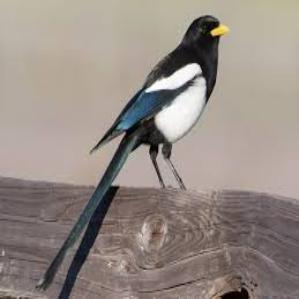
\includegraphics[width=1\linewidth]{18_6.jpg}
						
						% 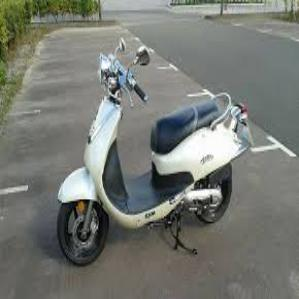
\includegraphics[width=1\linewidth]{670_6.jpg}
			
						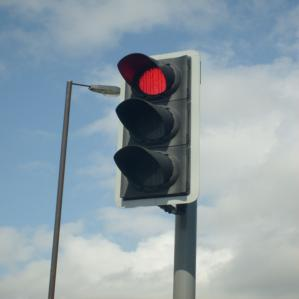
\includegraphics[width=1\linewidth]{920_55.jpg}
					\end{minipage}%
				}
				\subfigure[VGG16]{
					\begin{minipage}[b]{0.15\linewidth}
						\centering
						% 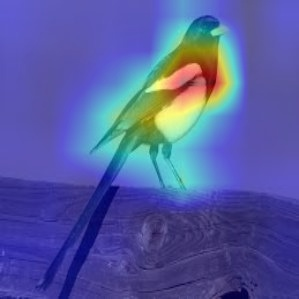
\includegraphics[width=1\linewidth]{18_6_vgg16.jpg}
						
						% 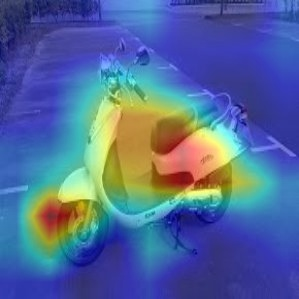
\includegraphics[width=1\linewidth]{670_6_vgg16.jpg}
			
						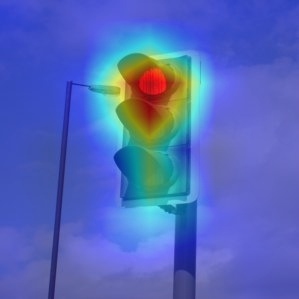
\includegraphics[width=1\linewidth]{920_55_vgg16.jpg}
					\end{minipage}%
				}
				\subfigure[VGG19]{
					\begin{minipage}[b]{0.15\linewidth}
						\centering
						% 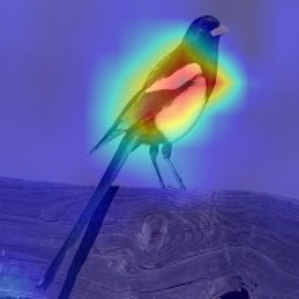
\includegraphics[width=1\linewidth]{18_6_vgg19.jpg}
						
						% 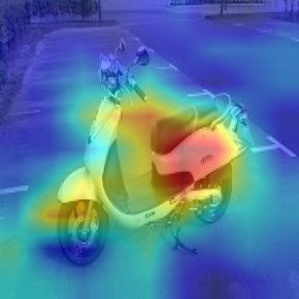
\includegraphics[width=1\linewidth]{670_6_vgg19.jpg}
			
						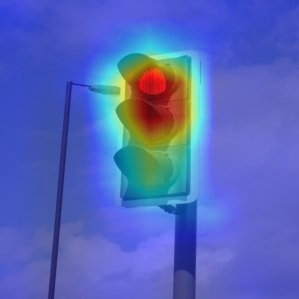
\includegraphics[width=1\linewidth]{920_55_vgg19.jpg}
					\end{minipage}%
				}
				\subfigure[ResNet50]{
					\begin{minipage}[b]{0.15\linewidth}
						\centering
						% 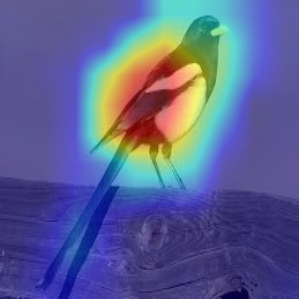
\includegraphics[width=1\linewidth]{18_6_resnet.jpg}
						
						% 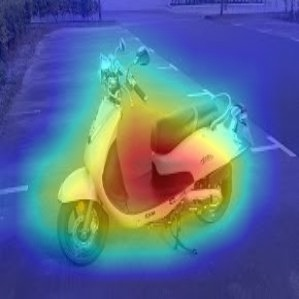
\includegraphics[width=1\linewidth]{670_6_resnet.jpg}
			
						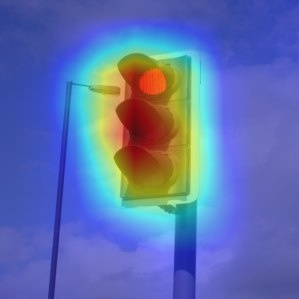
\includegraphics[width=1\linewidth]{920_55_resnet.jpg}
					\end{minipage}%
				}
				\subfigure[Inception-V3]{
					\begin{minipage}[b]{0.15\linewidth}
						\centering
						% 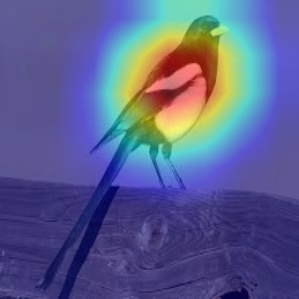
\includegraphics[width=1\linewidth]{18_6_incep.jpg}
						
						% 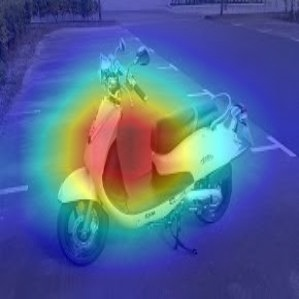
\includegraphics[width=1\linewidth]{670_6_incep.jpg}
			
						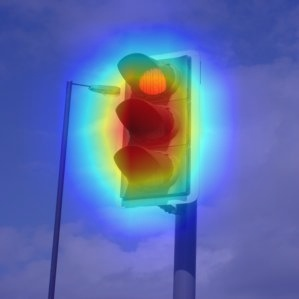
\includegraphics[width=1\linewidth]{920_55_incep.jpg}
					\end{minipage}%
				}}
				% \caption{Visualization of model interpretations using Grad-CAM on four well-known models: VGG16, VGG19, ResNet50, and Inception-V3.}
				% \label{fig:MI}
			\end{figure}
			\item Local adversarial perturbations still own weak transferability
		\end{itemize}
	\end{block}
	\begin{block}{Goals of This Paper}
		Generate local perturbations to fool the target model, while only requiring a small number of queries.
	\end{block}
\end{frame}
\begin{frame}
	\frametitle{DT Attack  ---  Methodology}

	\begin{block}{Dual Transferability}
		\begin{itemize}
			\item Transferability of local perturbations $\rightarrow$\emph{Warm start}
			\item Transferability of model interpretations$\rightarrow$\emph{Local perturbation}
			\end{itemize}
	\end{block}
	\begin{block}{Framework}
		\begin{figure}
			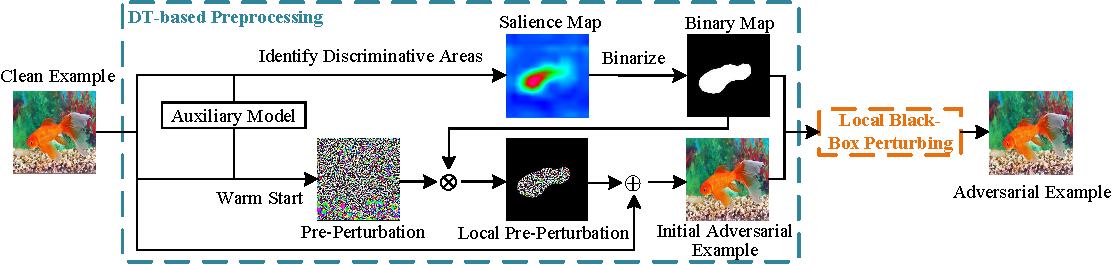
\includegraphics[width=\linewidth]{frame_1.pdf}
			% \caption{Framework of local and query-efficient black-box attack}
		\end{figure}
	\end{block}

	\alert{Make full use of auxiliary model to realize dual transferability}

	\begin{itemize}
			\item Li et al.\footnote{X. Li et al., ``Adversarial examples versus cloud-based detectors: A black-box empirical study,'' TDSC, 2021.} only considered determining the salience map
			\item Liu et al.\footnote{Y. Liu et al., ``Delving into transferable adversarial examples and black-box attacks,'' ICLR, 2017.} only considered enhancing the transferability of adversarial examples
	\end{itemize}
\end{frame}
\begin{frame}
	\frametitle{DT Attack --- Experiments}
	\begin{table}
		\centering	\footnotesize
		
		\caption{Overall evaluation}
		  % Table generated by Excel2LaTeX from sheet 'Sheet1'
		  \resizebox*{0.9\linewidth}{!}{
		\begin{tabular}{c|c|cccc|ccccc}
			\toprule
			\multirow{3}[6]{*}{Target} & \multirow{3}[6]{*}{Metric} & \multicolumn{4}{c|}{Gradient estimation} & \multicolumn{5}{c}{Random search} \\
			\cmidrule{3-11}      &       & \multicolumn{2}{c}{Global} & \multicolumn{2}{c|}{Local} & \multicolumn{2}{c}{Global} & \multicolumn{3}{c}{Local} \\
			\cmidrule{3-11}       &       & IFD   & NES   & DT-IFD & DT-NES & GS    & SimBA & SBLS  & DT-GS & DT-SimBA \\
			\midrule
			\multirow{4}[1]{*}{ResNet50} & NoQ $\downarrow$   & 35770 & 954   & 8377  &  660     & 452   & 5743  & 376   & 223   & 2526 \\
				& SR $\uparrow$    & 100\% & 47.56\% & 99.51\% &  65.85\%     & 97.80\% & 83.66\% & 97.80\% & 98.32\% & 87.56\% \\
				& PSNR $\uparrow$   & 38.99  & 42.77  & 40.09  &  43.00    & 32.49  & 47.24  & 32.94  & 36.44  & 42.70  \\
				& MAD $\downarrow$   & 8.72  & 25.81  & 11.10  &  27.41     & 51.65  & 22.85  & 37.04  & 30.29  & 25.63  \\
			\midrule
			\multirow{4}[2]{*}{Inception-V3} & NoQ $\downarrow$  & 65189 & 971   & 12627 &  733     & 895   & 5029  & 678   & 280   & 1739 \\
				& SR $\uparrow$   & 99.27\% & 42.93\% & 99.76\% &  73.66\%     & 83.66\% & 81.46\% & 89.02\% & 92.68\% & 83.17\% \\
				& PSNR $\uparrow$ & 42.11  & 40.66 & 34.33  &   33.95    & 31.94  & 43.30  & 32.75  & 31.92  & 33.95  \\
				& MAD $\downarrow$  & 9.27  & 12.86  & 29.18  &  20.79     & 64.84  & 21.14  & 48.64  & 48.45  & 25.79  \\
			\bottomrule
		\end{tabular}%
		}
	  \end{table}%
	  \begin{table}
		\caption{Evaluation on different local areas}
		% \label{tb:mi_case_all}
		\centering \footnotesize
		\resizebox*{0.9\linewidth}{!}{
	\begin{tabular}{c|c|cccccc}
		\toprule
		Category & Metric & MI-GS & NMI-GS & R0.2-GS & R0.4-GS & R0.6-GS & R0.8-GS \\
		\midrule
		\multirow{2}[2]{*}{Animal} & NoQ $\downarrow$   & 639   & 839   & 859   & 819   & 859   & 822 \\
			  & SR $\uparrow$   & 85.65\% & 61.30\% & 81.30\% & 80.86\% & 80.43\% & 82.17\% \\
		\midrule
		\multirow{2}[2]{*}{Transport} & NoQ $\downarrow$  & 681   & 917   & 829   & 834   & 875   & 814 \\
			  & SR $\uparrow$   & 92.15\% & 69.61\% & 87.15\% & 88.24\% & 90.19\% & 88.24\% \\
		\midrule
		\multirow{2}[2]{*}{Traffic sign} & NoQ $\downarrow$  & 998   & 1096  & 1203  & 1218  & 1079  & 1105 \\
			  & SR $\uparrow$   & 83.33\% & 55.13\% & 78.20\% & 82.05\% & 75.64\% & 75.64\% \\
		\bottomrule
		\end{tabular}%
		}
	\end{table}
	\alert{DT strategy is universal and can be applied to different types of black-box attacks for significantly reducing the query overhead}
\end{frame}
\subsection{EBRA}
\begin{frame}
	\frametitle{EBRA \footnote{Erase and repair: An efficient
	box-free removal attack on deep hiding. TIFS under review} --- Introduction}
	\begin{block}{Background \& Motivation}
		\begin{figure}
			\centering
			\setlength{\abovecaptionskip}{0.cm}
			\resizebox*{0.75\linewidth}{!}{
			\subfigure[DDH]{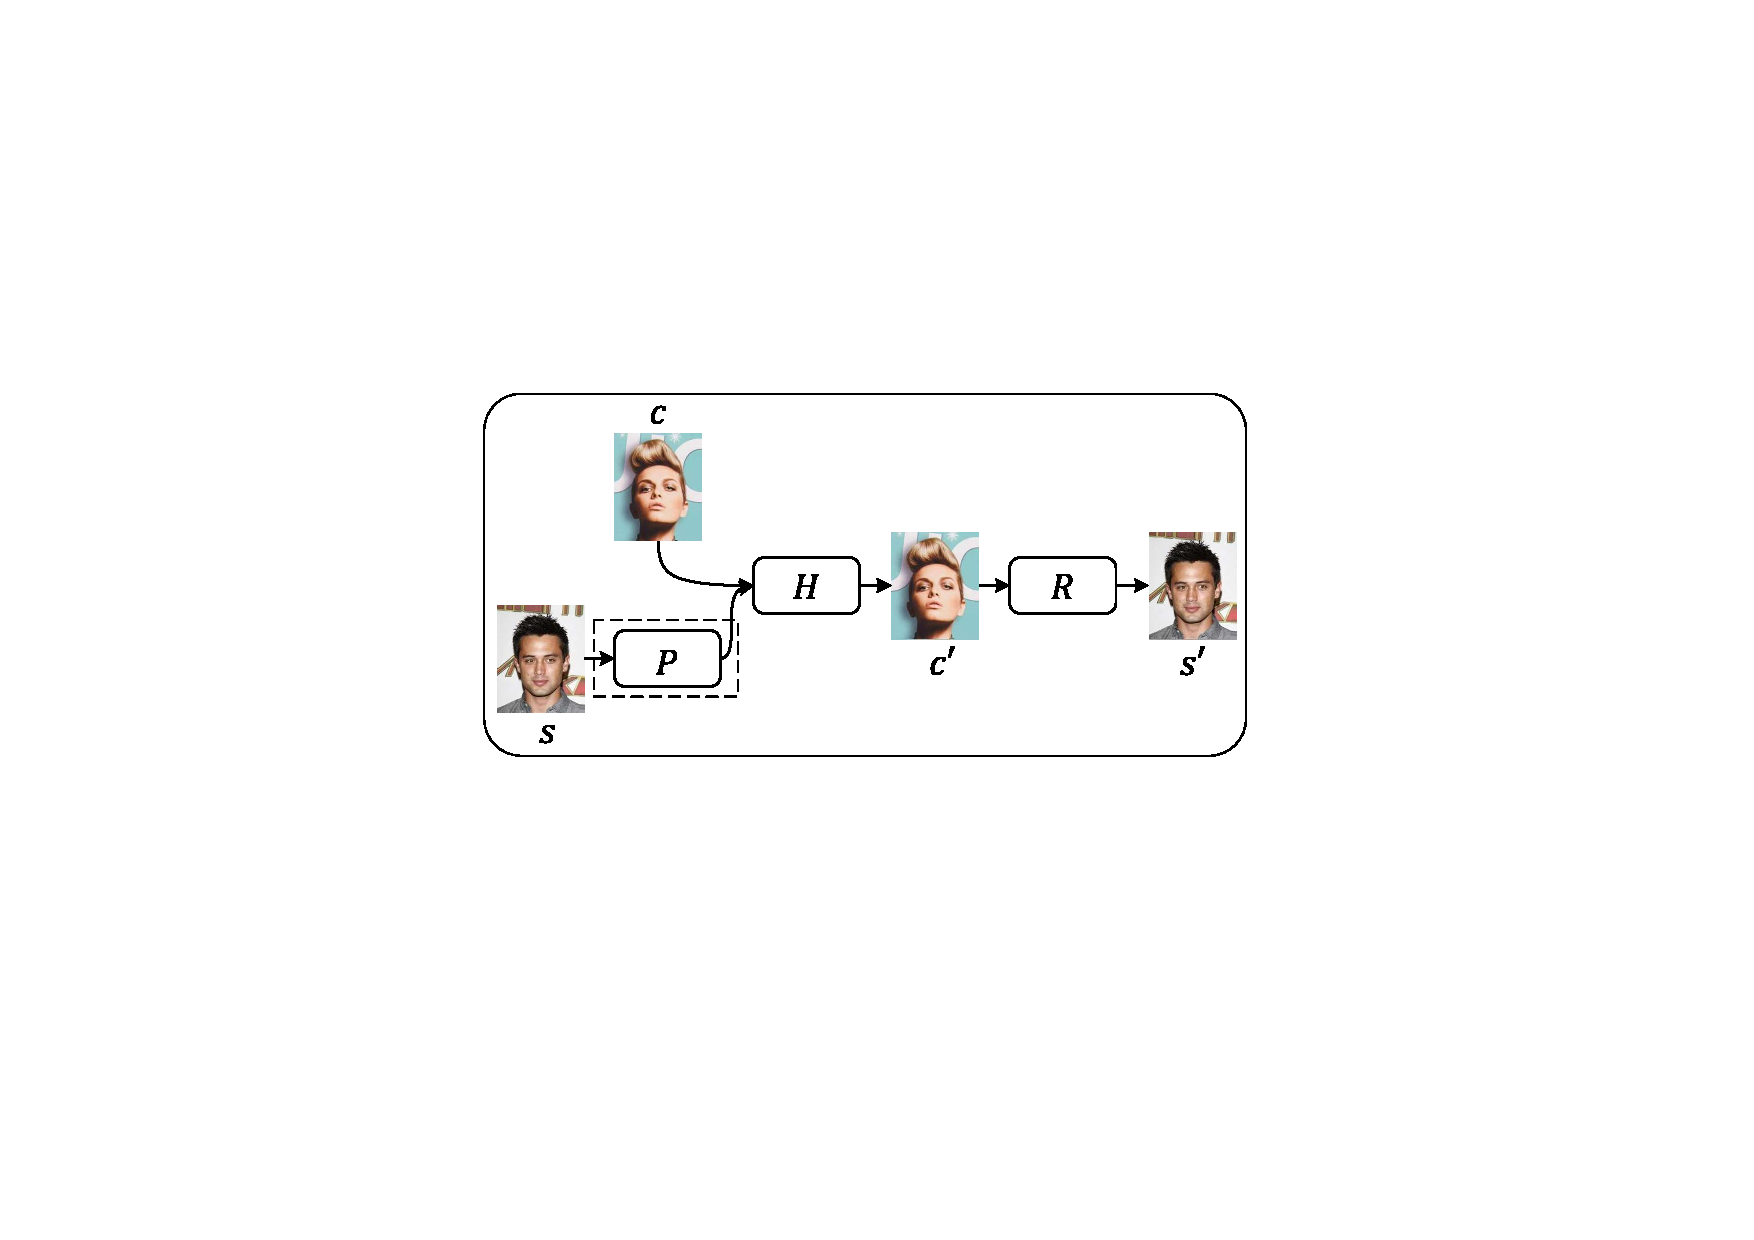
\includegraphics[width=0.35\linewidth]{DDH.pdf}}
			\subfigure[UDH]{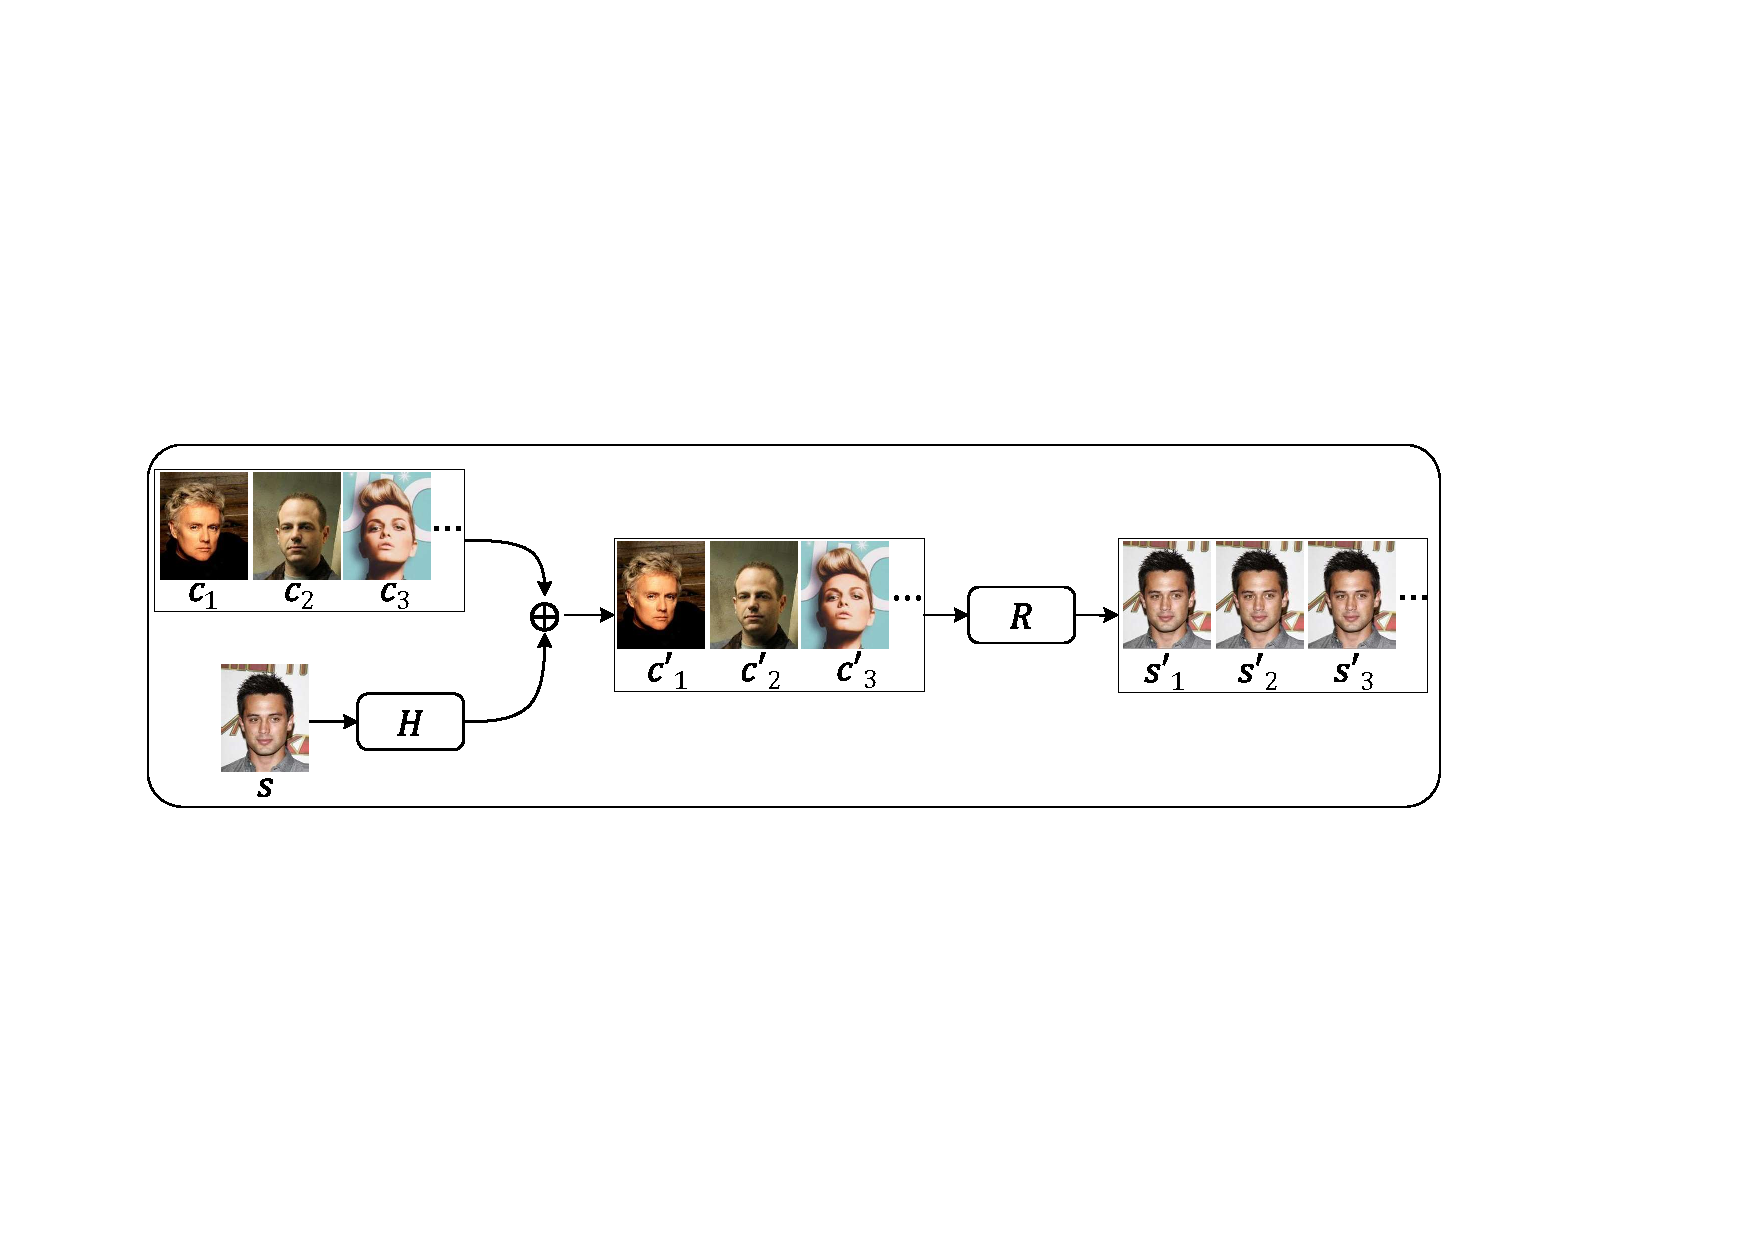
\includegraphics[width=0.59\linewidth]{UDH.pdf}}}
			% \caption{Meta-architectures of existing deep hiding. (a) the hiding network ($H$) in DDH is responsible for encoding the secret image $s$ and embedding the encoding results into the cover image $c$ at the same time; (b) the hiding network in UDH is only responsible for encoding the secret image and the encoding results can be hidden in arbitrary cover images by subsequent element-wise addition.}
			% \label{fig:meta-arch}
		\end{figure}
		Deep hiding significantly increases the message capacity and owns strong robustness. But we observe that existing deep hiding schemes have the following \alert{two vulnerabilities}:
		\begin{itemize}
			\item Locality
			\item Low redundancy
		\end{itemize}
	\end{block}
	\begin{block}{Goals of This Paper}
		Challenge the robustness of existing deep hiding schemes, including their enhanced versions. Specifically,
		\begin{itemize}
			\item Erase embedded secrets from container images
			\item Preserve the visual quality of container images
		\end{itemize}

	\end{block}
\end{frame}
\begin{frame}
	\frametitle{EBRA --- Methodology}
	\begin{block}{Framework}
		\begin{figure}
			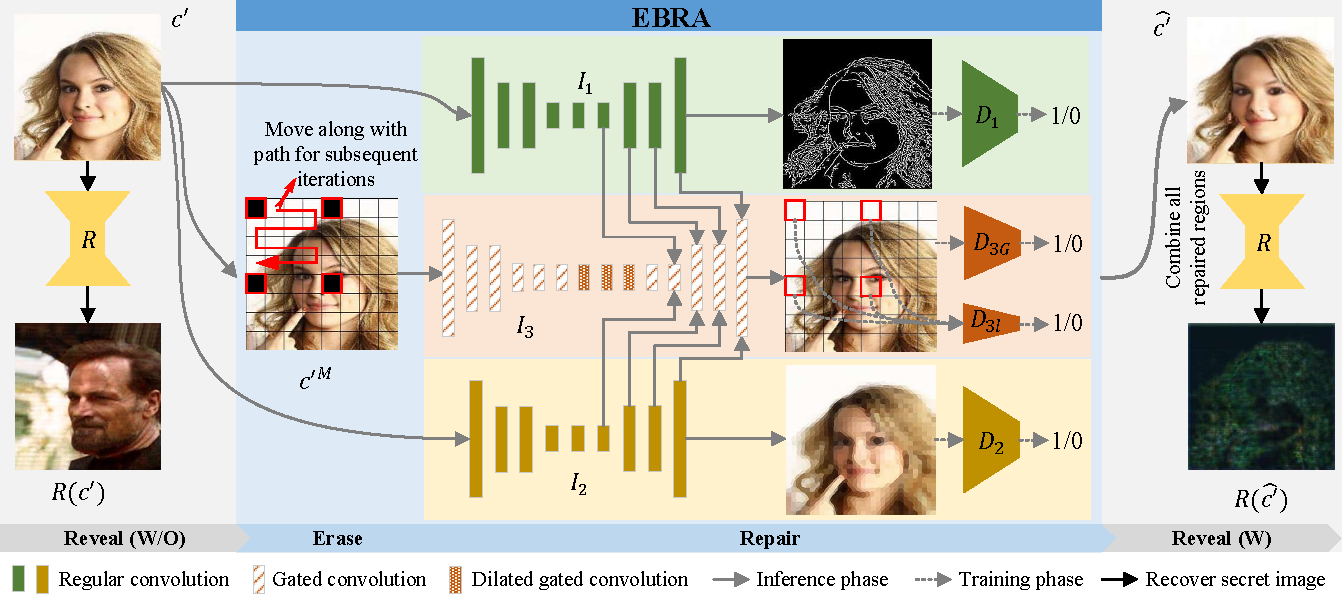
\includegraphics[width=0.8\linewidth]{ebra.pdf}
		\end{figure}
	\end{block}
	\alert{The auxiliary information (contour and color) does not provide erased secrets to the inpainting model and assists the inpainting model to repair the erased pixels}

\end{frame}
\begin{frame}
	\frametitle{EBRA --- Experiments}
	\begin{block}{Subjective Evaluation}
		\begin{table}[]
			\centering
			% \caption{Failure rate of all test methods in the subjective evaluation}
			\resizebox*{0.75\linewidth}{!}{
			\begin{tabular}{c|c|c|c|c|c|c|c}
			  \hline
			Attack & UDH   & UHD-GB & UDH-GN & UDH-Drop & UDH-JPEG                    & UDH-Quan                    & UDH-AE \\
			\hline
			GB     & 100\% & 100\%  & 100\%  & 100\%    & 100\%                       & 100\%                       & 100\%  \\
			GN     & 10\%  & 18\%   & 100\%  & 61\%     & 29\% & 86\% & 98\%   \\
			Drop   & 12\%  & 92\%   & 100\%  & 100\%    & 97\%                        & 45\%                        & 99\%   \\
			JPEG   & 97\%  & 100\%  & 100\%  & 5\%      & 100\%                       & 100\%                       & 100\%  \\
			MB     & 89\%  & 99\%   & 99\%   & 100\%    & 98\%                        & 97\%                        & 100\%  \\
			CD     & 100\% & 100\%  & 100\%  & 100\%    & 100\%                       & 100\%                       & 100\%  \\
			FPCA   & 99\%  & 100\%  & 100\%  & 100\%    & 100\%                       & 100\%                       & 100\%  \\
			% SHIELD & \textbf{0}\%   & \textbf{0}\%    & \textbf{0}\%    & \textbf{0}\%      & 3\%                         & 2\%                         & 16\%   \\
			PD     & 100\% & 100\%  & 100\%  & 100\%    & 100\%                       & 100\%                       & 100\%  \\
			BDR    & 27\%  & 46\%   & 100\%  & 65\%     & 25\%                        & 92\% & 100\%  \\
			NES    & 9\%   & 11\%   & 100\%  & 44\%     & 26\% & 89\% & 99\%   \\ \hline
			\textbf{EBRA}   & \textbf{0}\%   & \textbf{0}\%    & \textbf{0}\%    & \textbf{0}\%      & \textbf{1}\%     & \textbf{1}\%     & \textbf{3}\% \\ \hline
			\end{tabular}
			}
			\label{tab:subjective}
			\end{table}
	\end{block}
	\begin{block}{Objective Evaluation}
		\begin{table}
			\centering
			% \caption{Attack results on UDH and its enhanced versions}
			\resizebox*{0.75\linewidth}{!}{
			  \begin{tabular}{c|c|c|c|c|c|c|c}
				\hline
			     Attack & UDH           & UDH-GB        & UDH-GN        & UDH-Drop      & UDH-JPEG      & UDH-Quan      & UDH-AE        \\ \hline
				GB     & 0.709\textbar0.282 & 0.710\textbar0.657 & 0.611\textbar0.299 & 0.673\textbar0.150 & 0.695\textbar0.507 & 0.701\textbar0.123 & 0.616\textbar0.352 \\
				GN     & \underline{0.436\textbar0.043} & \underline{0.436\textbar0.040} & 0.430\textbar0.334 & 0.434\textbar0.066 & \underline{0.437\textbar0.047} & \underline{0.436\textbar0.037} & 0.432\textbar0.073 \\
				Drop   & \underline{0.750\textbar0.042} & 0.768\textbar0.064 & 0.646\textbar0.140 & 0.729\textbar0.377 & 0.790\textbar0.082 & 0.761\textbar0.054 & 0.694\textbar0.086 \\
				JPEG   & 0.842\textbar0.065 & 0.842\textbar0.080 & 0.695\textbar0.141 & \underline{0.780\textbar\textbf{0.012}} & 0.839\textbar0.536 & 0.831\textbar0.054 & 0.771\textbar0.268 \\
				% 												% & Quan   & \textbf{1.000}\textbar0.889 & \textbf{1.000}\textbar0.892 & \textbf{1.000}\textbar0.989 & \textbf{1.000}\textbar0.922 & \textbf{1.000}\textbar0.908 & \textbf{1.000}\textbar0.809 & \textbf{1.000}\textbar0.952 \\
				MB&0.441\textbar0.259&0.436\textbar0.330&0.384\textbar0.313&0.416\textbar0.299&0.428\textbar0.347&0.434\textbar0.214&0.405\textbar0.292\\
				CD&0.772\textbar0.745&0.773\textbar0.762&0.772\textbar0.804&0.772\textbar0.815&	0.773\textbar0.750&0.772\textbar0.767&0.774\textbar0.773\\
				% 												% &ET&0.227\textbar0.098&0.233\textbar0.131&0.206\textbar0.162&0.220\textbar0.144&0.233\textbar0.145&0.230\textbar0.100&0.214\textbar0.159\\
				FPCA&0.902\textbar0.570&0.900\textbar0.633&0.895\textbar0.750&0.908\textbar0.675&0.905\textbar0.627&0.907\textbar0.623&0.895\textbar0.679\\
				% 												% &RDG&\underline{0.084\textbar0.045}&\underline{0.084\textbar0.046}&0.072\textbar0.065&0.079\textbar0.058&0.085\textbar0.058&\underline{0.083\textbar0.049}&0.076\textbar0.064\\
				% 												% &SHIELD&\underline{0.653\textbar0.010}&\underline{0.654\textbar\textbf{0.012}}&\underline{0.574\textbar0.028}&\underline{0.622\textbar0.016}&\underline{0.659\textbar0.014}&\underline{0.649\textbar0.023}&0.616\textbar0.054\\
				PD&0.852\textbar0.417&0.853\textbar0.406&0.847\textbar0.796&0.854\textbar0.486&0.852\textbar0.430&0.853\textbar0.406&0.850\textbar0.524\\
				% 												% &FD&\underline{0.119\textbar0.039}&\underline{0.116\textbar0.040}&0.117\textbar0.107&0.114\textbar0.069&0.112\textbar0.062&\underline{0.120\textbar0.025}&0.085\textbar0.074\\
				BDR&0.508\textbar0.052&0.506\textbar0.055&0.505\textbar0.285&0.504\textbar0.077&0.507\textbar0.060&\underline{0.507\textbar0.050}&0.501\textbar0.108\\
				NES    & \underline{0.460\textbar0.040} & \underline{0.460\textbar0.040} & 0.453\textbar0.332 & 0.458\textbar0.066 & \underline{0.462\textbar0.045} & \underline{0.460\textbar0.036} & 0.457\textbar0.075 \\ \hline
				\textbf{EBRA}   & \underline{0.619\textbar\textbf{0.004}} & \underline{0.560\textbar\textbf{0.012}} & \underline{0.493\textbar\textbf{0.021}} & \underline{0.544\textbar0.016} & \underline{0.523\textbar\textbf{0.008}} & \underline{0.546\textbar\textbf{0.013}} & \underline{0.563\textbar\textbf{0.022}}\\ \hline
			  \end{tabular}
			}
		  \end{table}
	\end{block}
\end{frame}
\begin{frame}
	\frametitle{EBRA --- Experiments}
	\textbf{Visualization Examples}
	\begin{figure}
		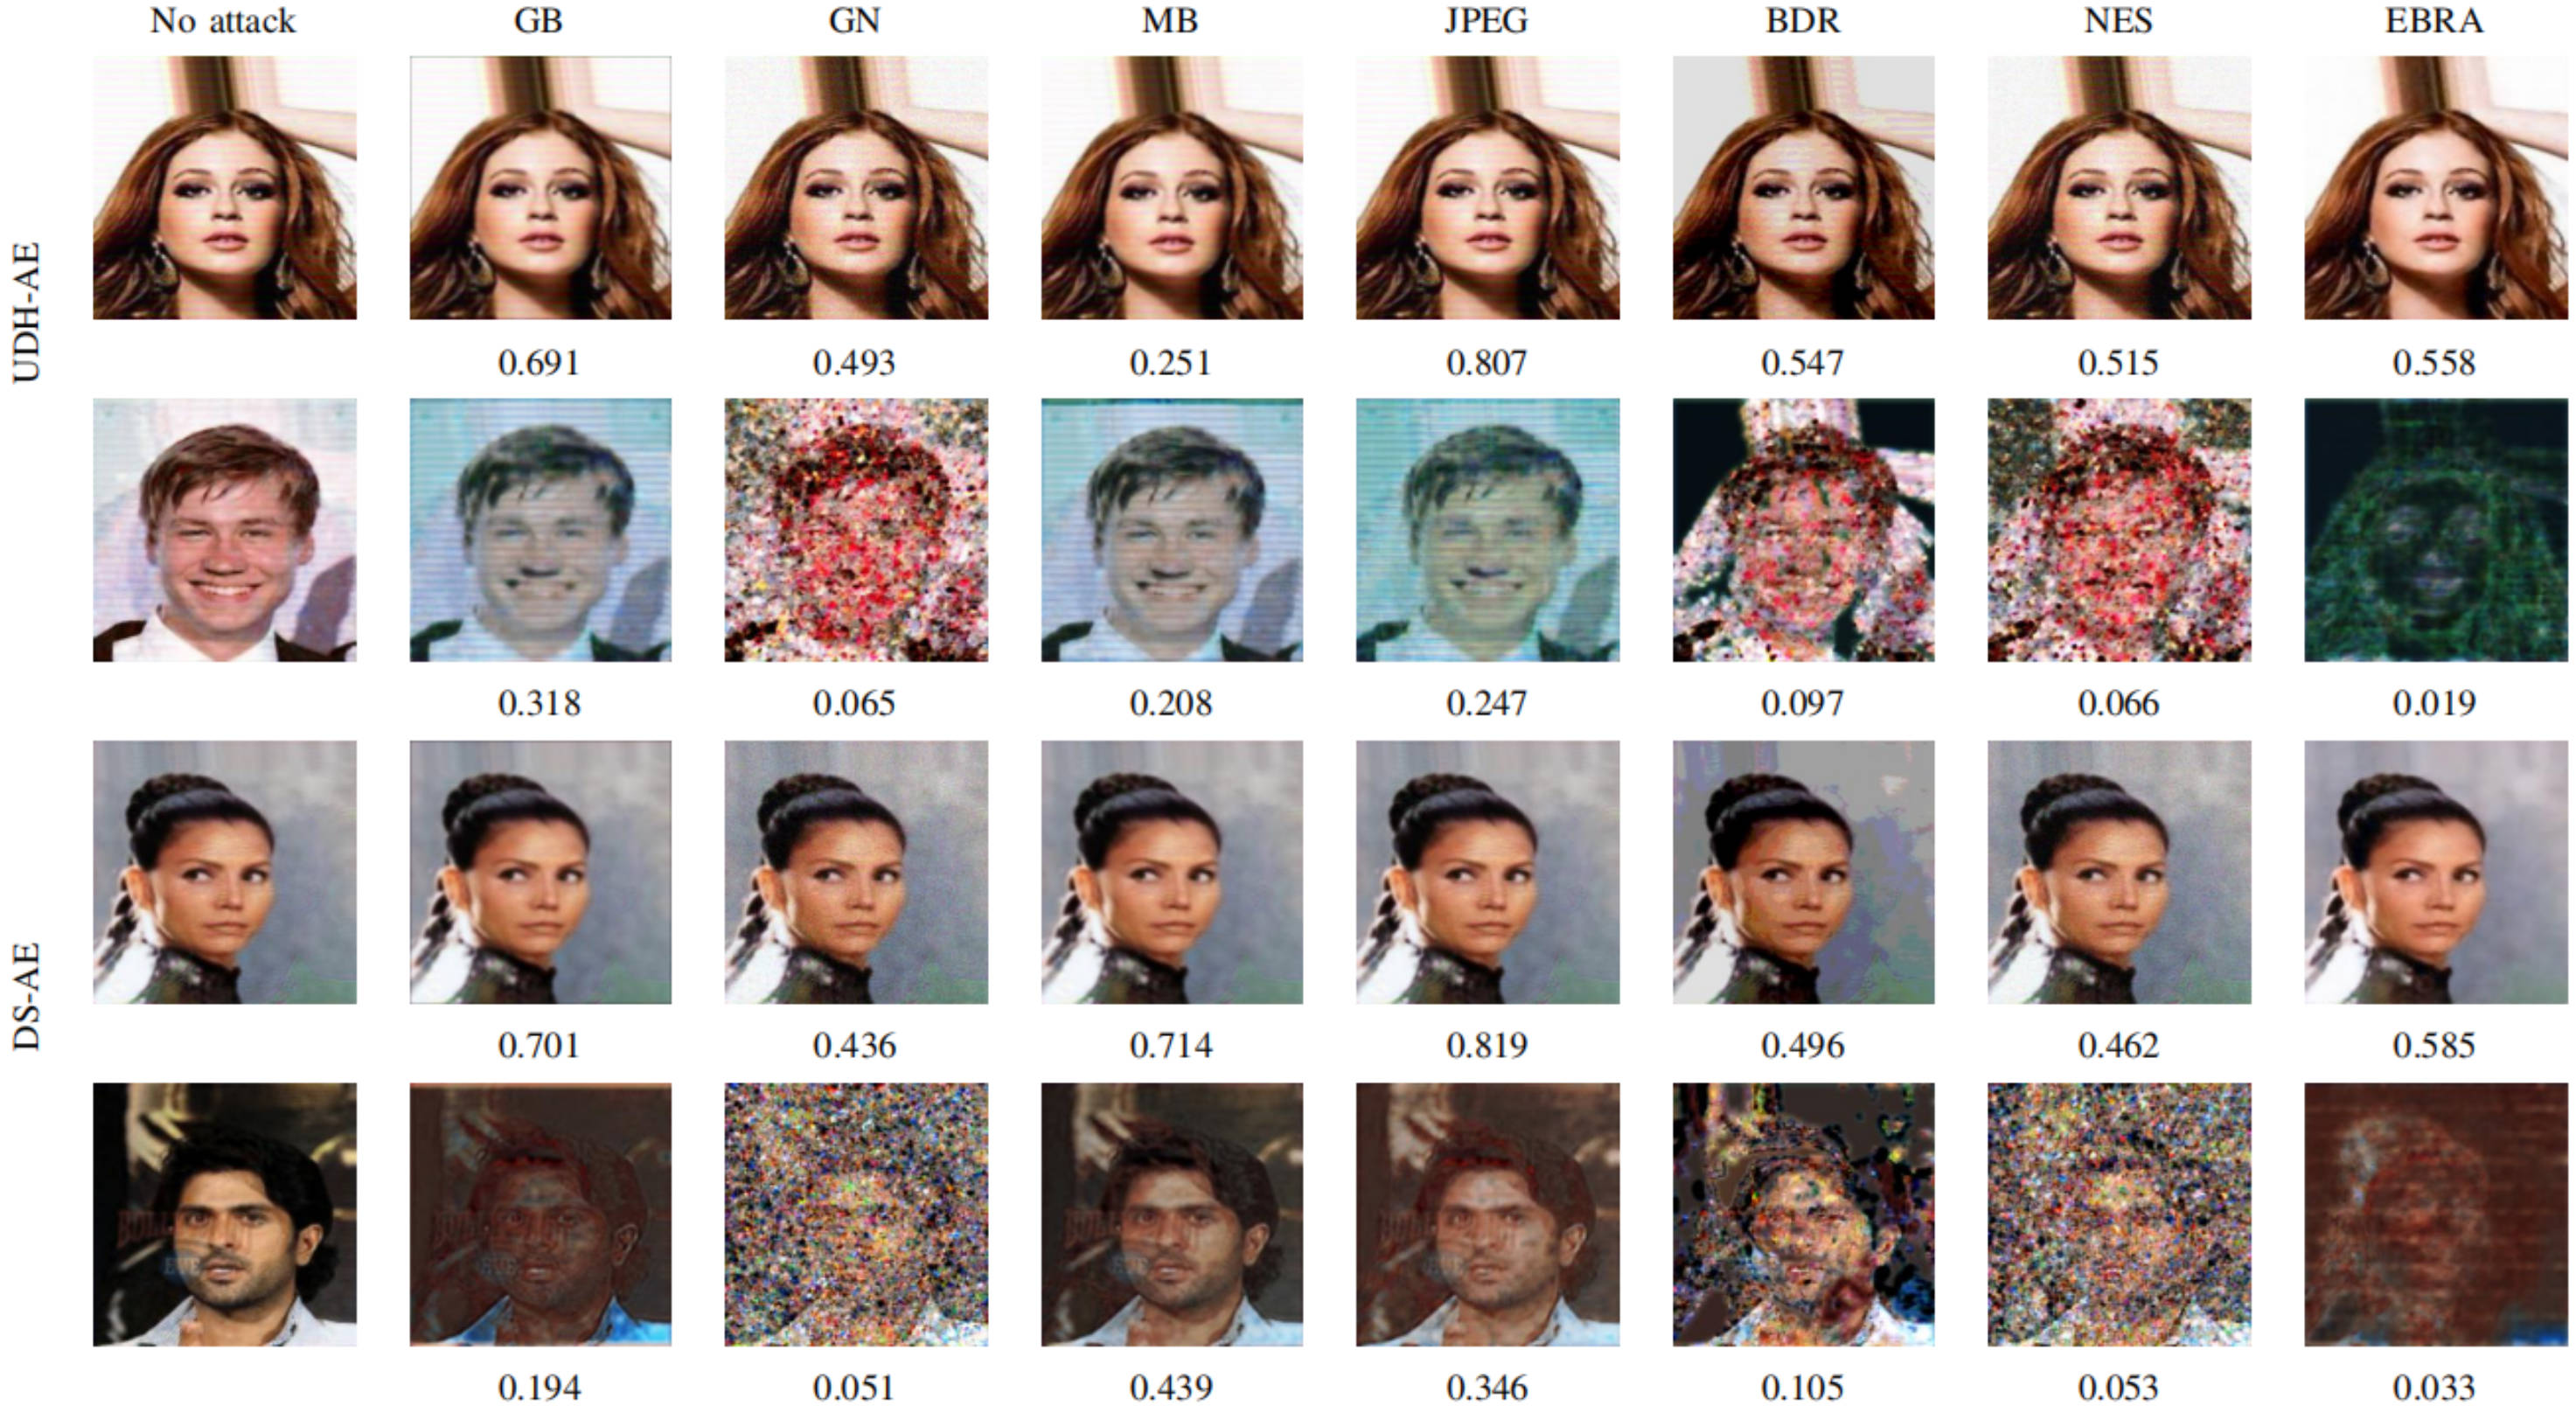
\includegraphics[width=0.9\linewidth]{ebra_visual.jpg}
	\end{figure}
	\alert{No valid secret information can be revealed after adopting EBRA to process container images.}
\end{frame}
\begin{frame}
	\frametitle{EBRA --- Experiments}
	\textbf{Attempts to Resist EBRA}

	\alert{If the defender understand all details of EBRA, including all involved parameters,} he can improve the robustness of the deep hiding models adversarially against EBRA through targeted adversarial training. 

	\alert{However, such improvement is limited.} We can still erase the embedded secrets using new models in EBRA, which are trained with new hyper-parameters.
	\begin{table}
		\centering
		%   \caption{Evaluation on more robust models}
		  \resizebox*{0.7\linewidth}{!}{
		  \begin{tabular}{c|c|c|c|c}
			\hline
			\multirow{2}{*}{Attack} & \multicolumn{2}{c|}{PSNR-C\textbar PSNR-S} & \multicolumn{2}{c}{VIF-C\textbar VIF-S} \\
		\cline{2-5}          & UDH-C & UDH-EBRA & UDH-C & UDH-EBRA \\
			\hline
			% EBRA  &  23.88$\textbar$10.51     & 24.43$\textbar$12.44 &   0.260$\textbar$0.014    & 0.293$\textbar$0.038 \\
			EBRA & 28.31\textbar10.67 & 29.43\textbar16.81 & 0.530\textbar0.015 & 0.569\textbar0.157 \\
			$\text{EBRA}^*$ & -     & 28.92\textbar11.97 & -     & 0.492\textbar0.036 \\
			\hline
			\end{tabular}%
		  \label{tab:udh_adv}%
		  }
	  \end{table}
	\alert{Adversarial training, even targeted adversarial training, is useless to resist EBRA.}
\end{frame}


% \subsection{Blocks}

% \begin{frame}
% 	\frametitle{Blocks of Highlighted Text}
	
% 	\begin{block}{Block Title}
% 		Lorem ipsum dolor sit amet, consectetur adipiscing elit. Integer lectus nisl, ultricies in feugiat rutrum, porttitor sit amet augue.
% 	\end{block}
	
% 	\begin{exampleblock}{Example Block Title}
% 		Aliquam ut tortor mauris. Sed volutpat ante purus, quis accumsan.
% 	\end{exampleblock}
	
% 	\begin{alertblock}{Alert Block Title}
% 		Pellentesque sed tellus purus. Class aptent taciti sociosqu ad litora torquent per conubia nostra, per inceptos himenaeos.
% 	\end{alertblock}
	
% 	\begin{block}{} % Block without title
% 		Suspendisse tincidunt sagittis gravida. Curabitur condimentum, enim sed venenatis rutrum, ipsum neque consectetur orci.
% 	\end{block}
% \end{frame}

% ---  ---  ---  ---  ---  ---  ---  ---  ---  ---  ---  ---  ---  ---  ---  ---  ---  ---  ---  ---  ---  ---  ---  --- 
\section{Future Work}
\begin{frame}
	tmp
\end{frame}


\begin{frame}[plain] % The optional argument 'plain' hides the headline and footline
	\begin{center}
		{\Huge \textbf{The End}}
		
		\bigskip\bigskip % Vertical whitespace
		
		{\LARGE \textbf{Thanks}}
	\end{center}
\end{frame}

% ---  ---  ---  ---  ---  ---  ---  ---  ---  ---  ---  ---  ---  ---  ---  ---  ---  ---  ---  ---  ---  ---  ---  ---  ---  ---  ---  ---  ---  ---  ---  ---  ---  ---  ---  ---  ---  ---  ---  ---  ---  ---  ---  --- 

\end{document} 